\documentclass[aspecttatio=169]{beamer}
\title{The Effects of Rotation on Stratified Turbulence}
\author[Dante Buhl]{Dante Buhl \\{\scriptsize Advised by: Pascale Garaud}}
\date{November 25, 2024}
\institute{UCSC Applied Mathematics}
\graphicspath{ {./images/} }
\usepackage{verbatim}
\usetheme{Dresden}
%\usecolortheme{spruce}
\usecolortheme{dolphin}
\usefonttheme{serif}

%%%%%%%%%%%%%%%%%%%%%%%%%%%%%%%%%%%%%%%%%%%%%%%%%%%%%%%%%%%%%%%%%%%%%%%%%%%%%%
% this code was copied from https://tex.stackexchange.com/a/516102
%%%%%%%%%%%%%%%%%%%%%%%%%%%%%%%%%%%%%%%%%%%%%%%%%%%%%%%%%%%%%%%%%%%%%%%%%%%%%%

\usepackage[bigfiles]{pdfbase}
\ExplSyntaxOn
\NewDocumentCommand\embedvideo{smm}{
  \group_begin:
  \leavevmode
  \tl_if_exist:cTF{file_\file_mdfive_hash:n{#3}}{
    \tl_set_eq:Nc\video{file_\file_mdfive_hash:n{#3}}
  }{
    \IfFileExists{#3}{}{\GenericError{}{File~`#3'~not~found}{}{}}
    \pbs_pdfobj:nnn{}{fstream}{{}{#3}}
    \pbs_pdfobj:nnn{}{dict}{
      /Type/Filespec/F~(#3)/UF~(#3)
      /EF~<</F~\pbs_pdflastobj:>>
    }
    \tl_set:Nx\video{\pbs_pdflastobj:}
    \tl_gset_eq:cN{file_\file_mdfive_hash:n{#3}}\video
  }
  %
  \pbs_pdfobj:nnn{}{dict}{
    /Type/RichMediaInstance/Subtype/Video
    /Asset~\video
    /Params~<</FlashVars (
      source=#3&
      skin=SkinOverAllNoFullNoCaption.swf&
      skinAutoHide=true&
      skinBackgroundColor=0x5F5F5F&
      skinBackgroundAlpha=0
    )>>
  }
  %
  \pbs_pdfobj:nnn{}{dict}{
    /Type/RichMediaConfiguration/Subtype/Video
    /Instances~[\pbs_pdflastobj:]
  }
  %
  \pbs_pdfobj:nnn{}{dict}{
    /Type/RichMediaContent
    /Assets~<<
      /Names~[(#3)~\video]
    >>
    /Configurations~[\pbs_pdflastobj:]
  }
  \tl_set:Nx\rmcontent{\pbs_pdflastobj:}
  %
  \pbs_pdfobj:nnn{}{dict}{
    /Activation~<<
      /Condition/\IfBooleanTF{#1}{PV}{XA}
      /Presentation~<</Style/Embedded>>
    >>
    /Deactivation~<</Condition/PI>>
  }
  %
  \hbox_set:Nn\l_tmpa_box{#2}
  \tl_set:Nx\l_box_wd_tl{\dim_use:N\box_wd:N\l_tmpa_box}
  \tl_set:Nx\l_box_ht_tl{\dim_use:N\box_ht:N\l_tmpa_box}
  \tl_set:Nx\l_box_dp_tl{\dim_use:N\box_dp:N\l_tmpa_box}
  \pbs_pdfxform:nnnnn{1}{1}{}{}{\l_tmpa_box}
  %
  \pbs_pdfannot:nnnn{\l_box_wd_tl}{\l_box_ht_tl}{\l_box_dp_tl}{
    /Subtype/RichMedia
    /BS~<</W~0/S/S>>
    /Contents~(embedded~video~file:#3)
    /NM~(rma:#3)
    /AP~<</N~\pbs_pdflastxform:>>
    /RichMediaSettings~\pbs_pdflastobj:
    /RichMediaContent~\rmcontent
  }
  \phantom{#2}
  \group_end:
}
\ExplSyntaxOff


\usepackage{amsmath}
\usepackage{pifont} \usepackage{hyperref}
\usepackage{amsthm} %proof environment
\usepackage{amssymb}
\usepackage{amsfonts}
%\usepackage{enumitem} %nice lists
\usepackage{verbatim} %useful for something 
\usepackage{xcolor}
\usepackage{blindtext} % I have no idea what this is 
\usepackage{caption}  % need this for unnumbered captions/figures
\usepackage{soul} % need this for the hl command
\usepackage{graphicx} % Required for inserting images
\usepackage{multimedia}
\usepackage{natbib}

\begin{document}

\newcommand{\wrms}{w_{\text{rms}}}
\newcommand{\bs}[1]{\boldsymbol{#1}}
\newcommand{\tb}[1]{\textbf{#1}}
\newcommand{\bmp}[1]{\begin{minipage}{#1\textwidth}}
\newcommand{\emp}{\end{minipage}}
\newcommand{\R}{\mathbb{R}}
\newcommand{\C}{\mathbb{C}}
\newcommand{\N}{\mathcal{N}}
\newcommand{\K}{\bs{\mathrm{K}}}
\newcommand{\m}{\bs{\mu}_*}
\newcommand{\s}{\bs{\Sigma}_*}
\newcommand{\dt}{\Delta t}
\newcommand{\dx}{\Delta x}
\newcommand{\tr}[1]{\text{Tr}(#1)}
\newcommand{\Tr}[1]{\text{Tr}(#1)}
\newcommand{\Div}{\nabla \cdot}
\renewcommand{\div}{\nabla \cdot}
\newcommand{\Curl}{\nabla \times}
\newcommand{\Grad}{\nabla}
\newcommand{\grad}{\nabla}
\newcommand{\grads}{\nabla_s}
\newcommand{\gradf}{\nabla_f}
\newcommand{\xs}{\bs{x}_s}
\newcommand{\xf}{\bs{x}_f}
\newcommand{\ts}{t_s}
\newcommand{\tf}{t_f}
\newcommand{\pt}{\partial t}
\newcommand{\pz}{\partial z}
\newcommand{\uvec}{\bs{u}}
\newcommand{\F}{\bs{F}}
\newcommand{\T}{\tilde{T}}
\newcommand{\ez}{\bs{e}_z}
\newcommand{\ex}{\bs{e}_x}
\newcommand{\ey}{\bs{e}_y}
\newcommand{\eo}{\bs{e}_{\bs{\Omega}}}
\newcommand{\ppt}[1]{\frac{\partial #1}{\partial t}}
\newcommand{\ppts}[1]{\frac{\partial #1}{\partial t_s}}
\newcommand{\pptf}[1]{\frac{\partial #1}{\partial t_f}}
\newcommand{\ppz}[1]{\frac{\partial #1}{\partial z}}
\newcommand{\ddz}[1]{\frac{d #1}{d z}}
\newcommand{\ppzetas}[1]{\frac{\partial^2 #1}{\partial \zeta^2}}
\newcommand{\ppzs}[1]{\frac{\partial #1}{\partial z_s}}
\newcommand{\ppzf}[1]{\frac{\partial #1}{\partial z_f}}
\newcommand{\ppx}[1]{\frac{\partial #1}{\partial x}}
\newcommand{\ppy}[1]{\frac{\partial #1}{\partial y}}
\newcommand{\ppzeta}[1]{\frac{\partial #1}{\partial \zeta}}


\begin{comment}
    1. Intro 
    2. Model
        - new forcing mechanism
    3. Previous Work?
        - Multiscale theory by Chini et al and Shahe et al
    4. Stochastically forced Stratified TurbulenceA
        - new horizontal structures in the flow
        - weak correlation between vertical vorticity and mixing
        - previous wmrs scalings aren't as effective
    5. Rotating Stratified Turbulence
        - new flow structures (columns appear in the flow)
        - mixinng is localized to anti-cyclones
        - inverse energy cascade to small horizontal wavenumbers
        - decline in vertical mixing 
        
\end{comment}

\frame{\titlepage}


\begin{frame}{Motivation}

\begin{itemize}
{\small
\item Stratified turbulence is a crucial phenomenon responsible for mixing and
transport in geophysical and astrophysical fluid dynamics. 

\item In relevant geophysical and astrophysical flows, both stratification and
rotation influence dynamics. 
} %end small
\end{itemize}

%\bmp{.49}
    %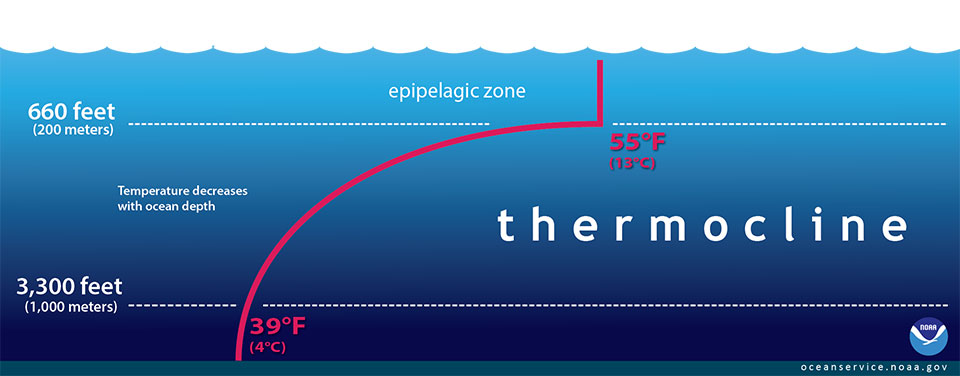
\includegraphics[width=\textwidth]{ocean_thermocline_NOS_NOAA.jpg}
%\emp

\end{frame}





%By contrast, Rotation barotropic structues wihch are invariant along the
%axis of rotation. (show pictures of cylinders)


\begin{frame}{Motivation}
\bmp{.47}
    {\footnotesize
    Nonrotating stratified turbulence is characterized by strongly
    anisotropic pancake structures within the flow. 
    \begin{figure}
        \centering
        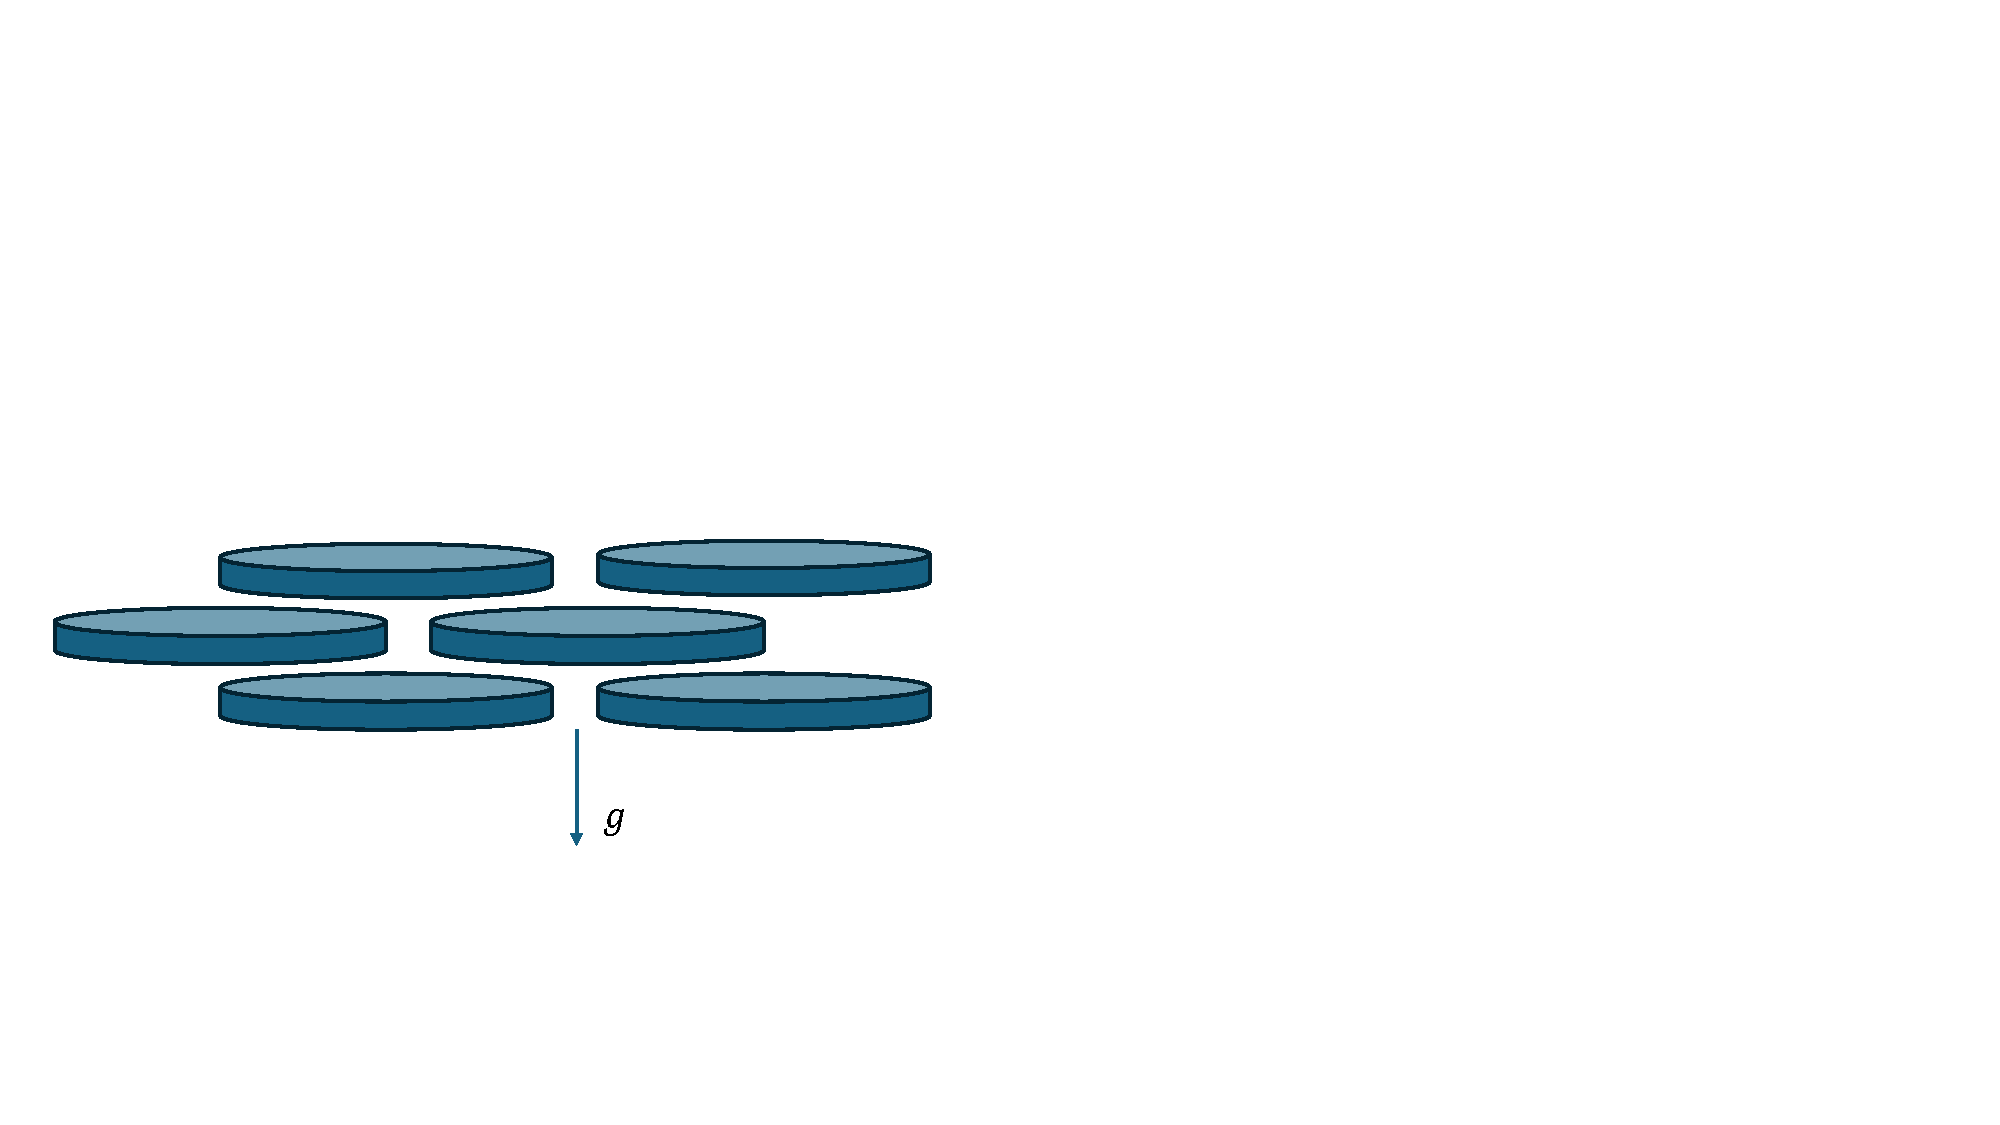
\includegraphics[width=.9\textwidth]{images/pancakes.pdf}
    \end{figure}
    } %end small
\emp
\hspace{6pt}
\bmp{.47}
    {\footnotesize
    Rotation promotes barotropic structures which are invariant along the axis
    of rotation.
    
    \begin{figure}
        \centering
        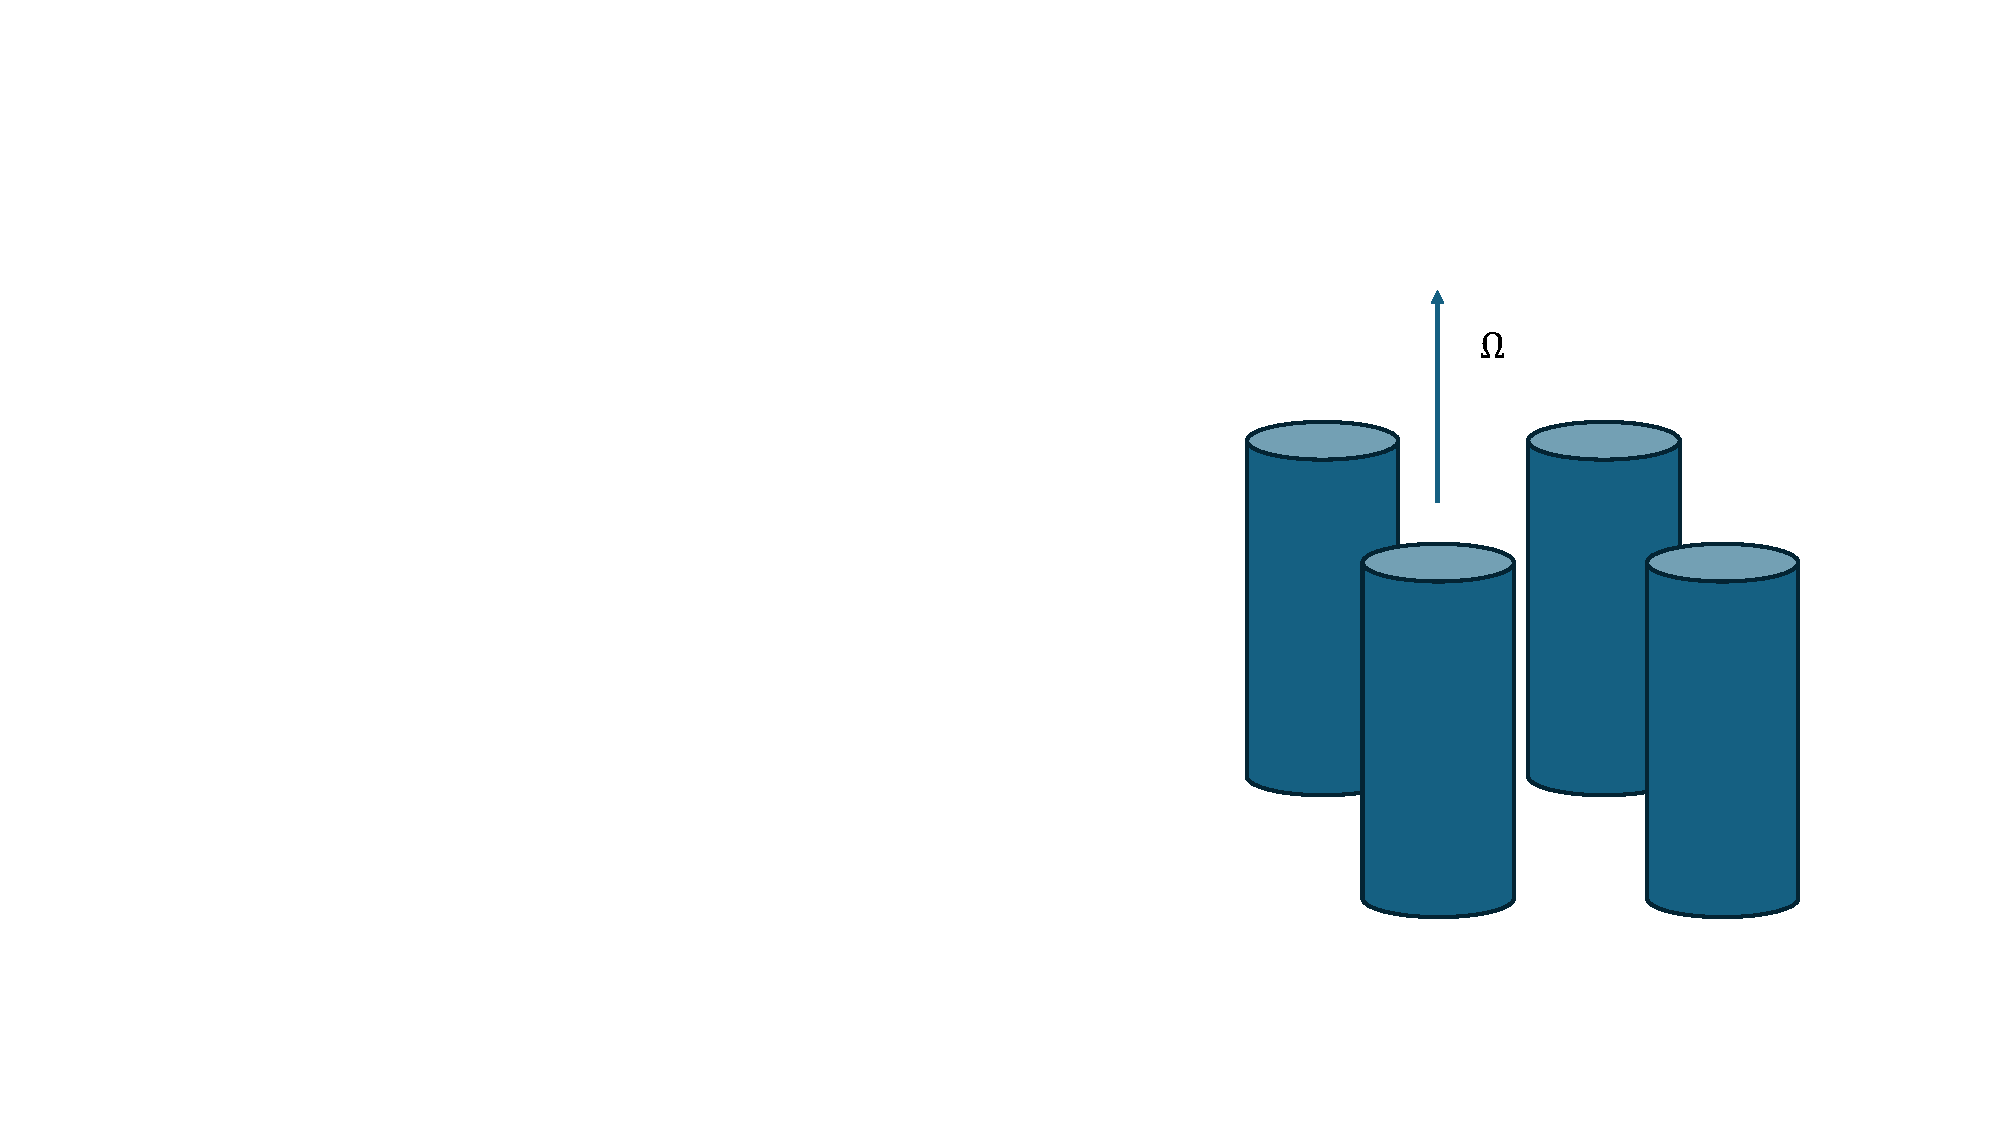
\includegraphics[width=.9\textwidth]{images/cylinders.pdf}
    \end{figure}
    } %end small
\emp

\vspace{10pt}

% This is the main question which we will attempt to answer. Maybe put it on its
% own slide.
Using DNS, we will study the competing effects of rotation and
stratification on vertical mixing in the flow. 

\end{frame}

\begin{frame}{Schematic}
    We condider a tripply periodic domain: 
    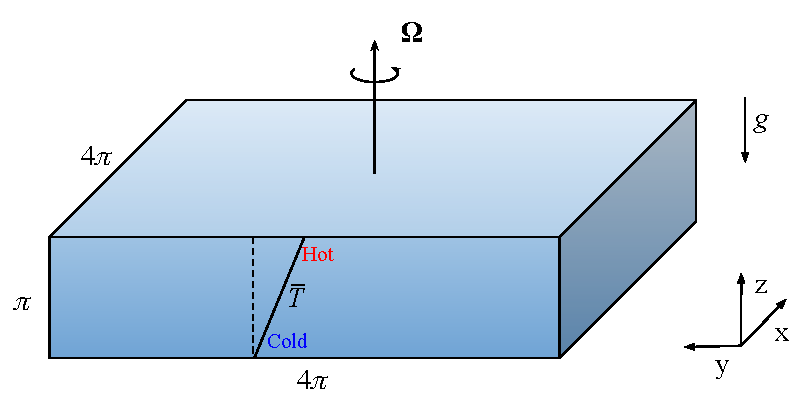
\includegraphics[width = \textwidth]{images/schematic.pdf}

    %\hl{add temp profile, gravity}
    % Notes: Tripply Periodic Domain with dimensions 4pi x 4pi x pi. We notice
    % the rotation vector omega placed in the diagram to visualize the angle of
    % rotation with respect to gravity (or the vertical coordinate direction).
    % It should also be noted that the rotation vector should be pointing in the
    % y direction. 
    % For the results you will be seeing today, rotation has not yet been
    % included, but it is the next step for our parameter study. 
\end{frame}

\begin{frame}{Governing Equations}

    {\small
    \begin{align}
        \ppt{\bs{u}} + \uvec \cdot \Grad \uvec +
        \frac{1}{Ro}(\ez \times
        \uvec) &= -\Grad p +
        \frac{T}{Fr^2}\ez + \F + \frac{1}{Re}\Grad^2\uvec \tag{mom.}\label{eq:momentum}\\
        \ppt{T} + \bs{u} \cdot \Grad T + w &= \frac{1}{Pe}\Grad^2T \tag{temp.} \label{eq:temp} \\
        \Div \bs{u} &= 0 \tag{cont.}\label{eq:cont}
    \end{align}
    
    \begin{align*}
        Re = \frac{UL}{\nu}, \quad Pe = \frac{UL}{\kappa}, \quad Fr =
        \frac{U}{NL}, \quad Ro = \frac{U}{2\Omega L}
    \end{align*}
    In what follows, simulations will be conducted with $Re = 600$ and $Pe = 60$
    ($Pr = 0.1$).
    }
    %\begin{itemize}
        %\item $U$ is the characteristic velocity
        %\item $L$ is the large eddy horizontal length scale
        %\item $N$ is the buoyancy frequency ($N = \sqrt{\alpha_Tg\ddz{\bar{T}}}$)
        %\item $\Omega$ is the angular velocity
        %\item $(\nu, \kappa)$ are the (viscous, thermal) diffusivity coefficients
    %\end{itemize}
    %Where $U$ is the characteristic velocity, $L$ is the eddy length scale, $N$ is the buoyancy frequency, and $\Omega$ is the angular velocity of the rotating body. 
    % Notes: Classic Non-dimensionalized Boussinesue Rotations which include a
    % buopyancy field, viscous and dissipative dynamics, as well as rotation
    % (the coriolis force). Thus we see the appearnce of the Rossby, Froude,
    % Reynolds, and Peclet numbers in the governing equations. It should b
    % mentioned that this rotation vector r = <0, sin(\phi), cos(\phi)>. 

\end{frame}

\begin{frame}{Forcing Mechanism}

    We choose the forcing to be purely horizontal and divergence-free stochastic
    process:
    \[
        \bs{F} = F_x\ex + F_y\ey, \quad \grad \cdot \bs{F} = 0
    \]
    The forcing is applied in spectral space and satisfies $\bs{k} \cdot \hat{\bs{F}} = 0$:
    \begin{gather*}
        \hat{F}_x = \frac{k_y}{|\bs{k}_h|}G(\bs{k}_h,t), \quad \hat{F}_y = \frac{-k_x}{|\bs{k}_h|}G(\bs{k}_h,t)\\
    \end{gather*}
    where $G(\bs{k}_h,t)$ is a Gaussian process of amplitude 1 and correlation
    timescale 1, and $|\bs{k}_h| \le \sqrt{2}$. 


\end{frame}

% what are the flow structures that we obtain?
\begin{frame}{Non-Rotating Stratified Turbulence}
    % Ux rms figure
    % plot info: B100 is -3.5:3.5
    % B300 is -5:5
    % B10 is -3:3
    %B1 is -5:5
    \centering

    Decreasing the Froude number creates increasingly anisotropic structures in
    $u$. 

    \vspace{5pt}

    \bmp{.235}
        \centering
       
        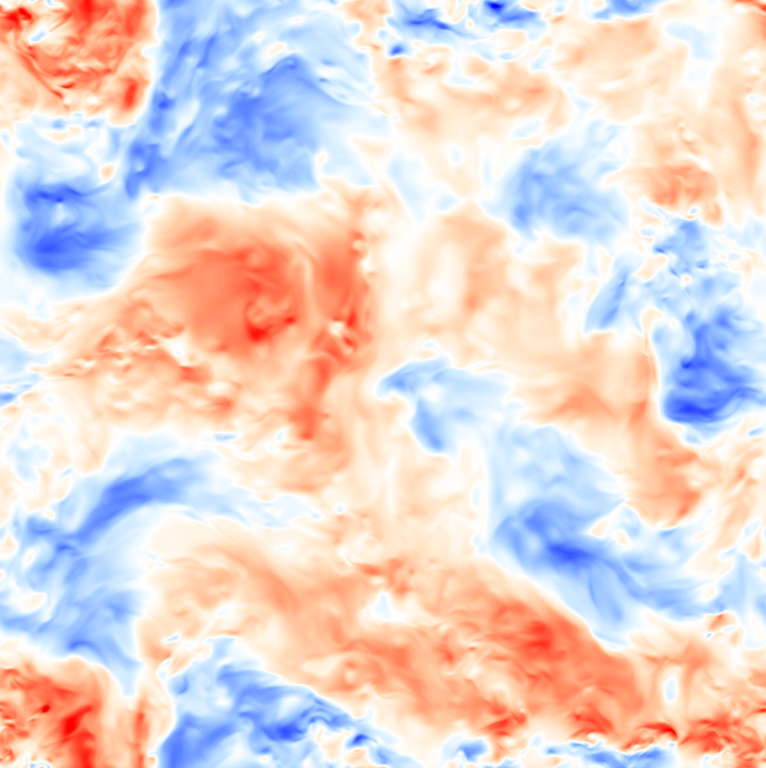
\includegraphics[width=\textwidth]{images/XYB1ux.png}
        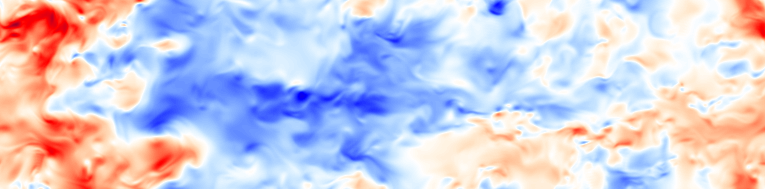
\includegraphics[width=\textwidth]{images/XZB1ux.png}
        \vspace{2pt}
        $1/Fr = 1$
        %\includegraphics[width = \textwidth]{images/B1Spec.pdf}
    \emp
    \hspace{1pt}
    \bmp{.235}
        \centering
        
        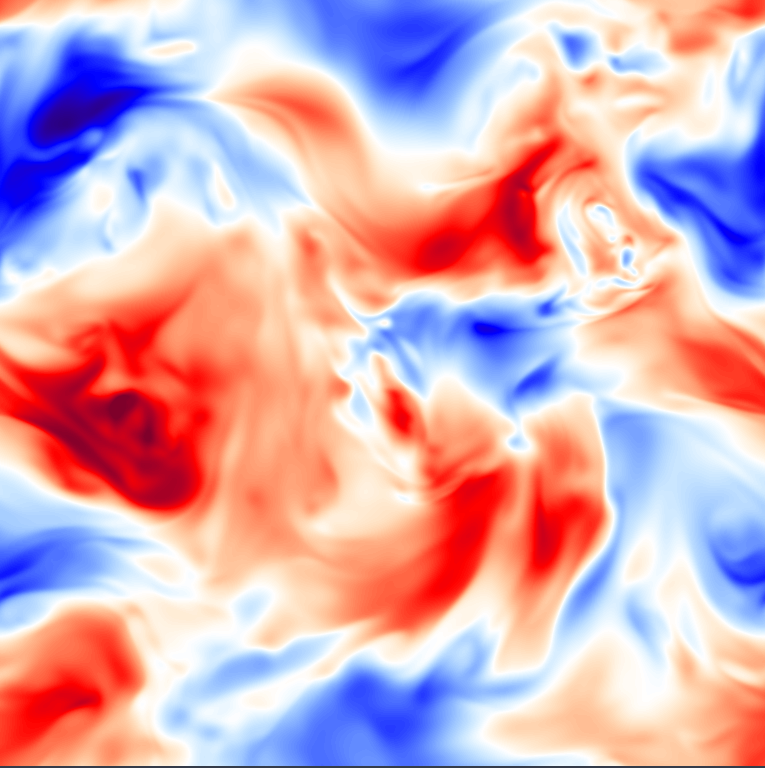
\includegraphics[width=\textwidth]{images/XYB10ux.png}
        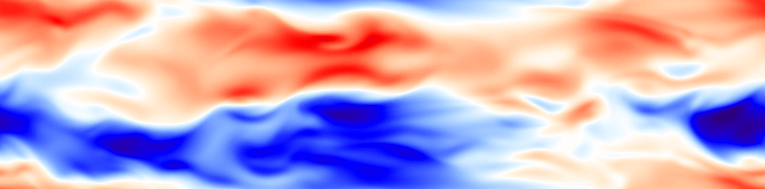
\includegraphics[width=\textwidth]{images/XZB10ux.png}
        \vspace{2pt}
        $1/Fr = 3.16$
        %\includegraphics[width = \textwidth]{images/B10Spec.pdf}
    \emp
    \hspace{1pt}
    \bmp{.235}
        \centering
        
        \includegraphics[width=\textwidth]{images/XYB100ux.png}
        \includegraphics[width=\textwidth]{images/XZB100ux.png}
         \vspace{2pt}
        $1/Fr = 10$
       %\includegraphics[width = \textwidth]{images/B100Spec.pdf}
    \emp
    \hspace{1pt}
    \bmp{.235}
        \centering
        
        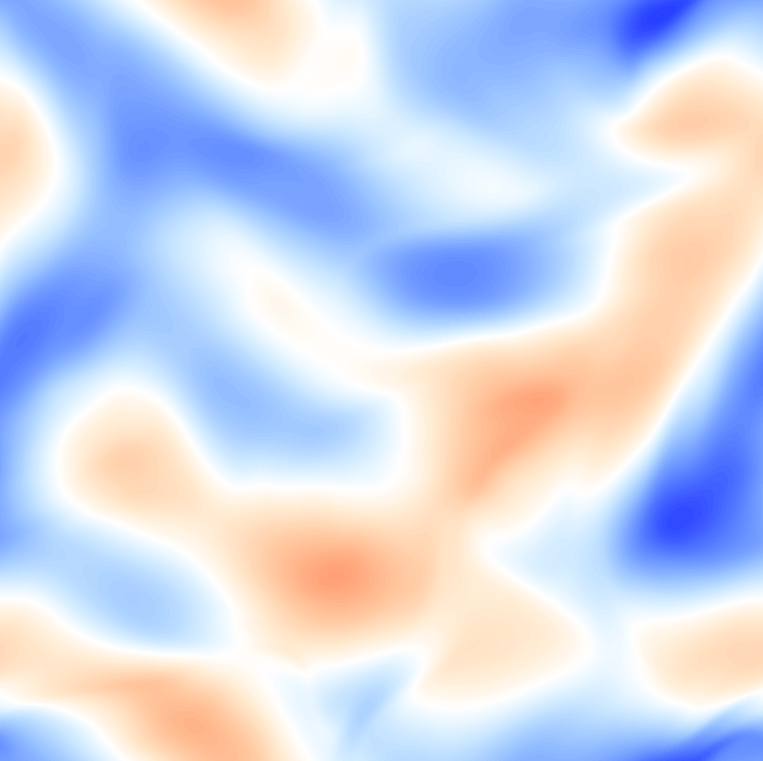
\includegraphics[width=.99\textwidth]{images/XYB300ux.png}
        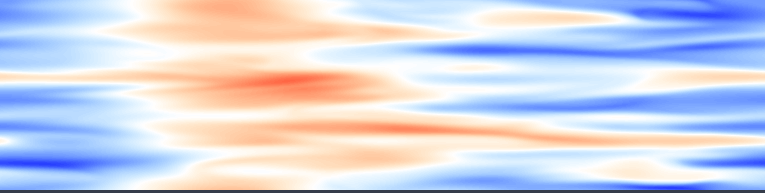
\includegraphics[width=.99\textwidth]{images/XZB300ux.png}
        \vspace{2pt}
        $1/Fr = 17.36$

        %\includegraphics[width = \textwidth]{images/B300Spec.pdf}
    \emp

    \[\overrightarrow{\rm Stratification}\]
\end{frame}

\begin{frame}{Rotating Stratified Turbulence at fixed $Fr = 0.18$}
    \centering

   \bmp{.33}
        Evolution of $\omega_z$
   \emp
   \bmp{.33}
        \centering
        $1/Ro = 0.5$
        \vspace{2pt}
        \embedvideo*{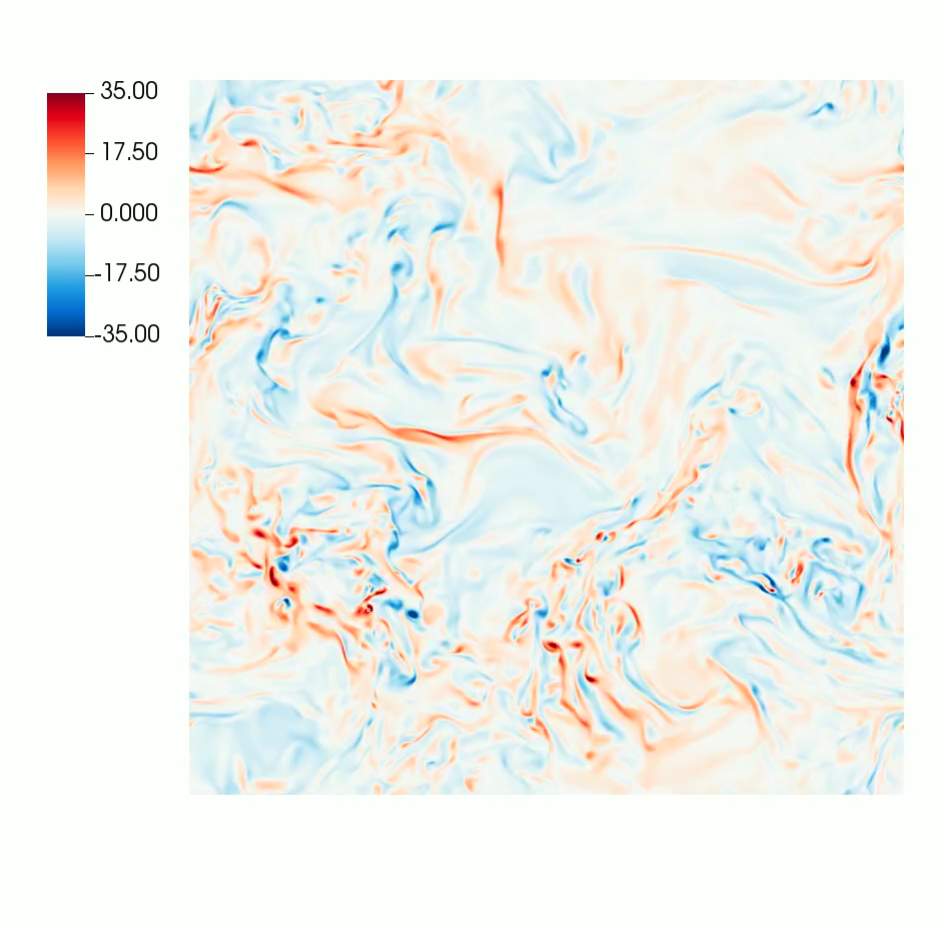
\includegraphics[width=.8\textwidth]{images/SC_Om0.5B30_XY.png}}{images/Om0.5B30_XY.mp4}
        \vspace{5pt}
        $1/Ro = 2$
        \vspace{2pt}
        \embedvideo*{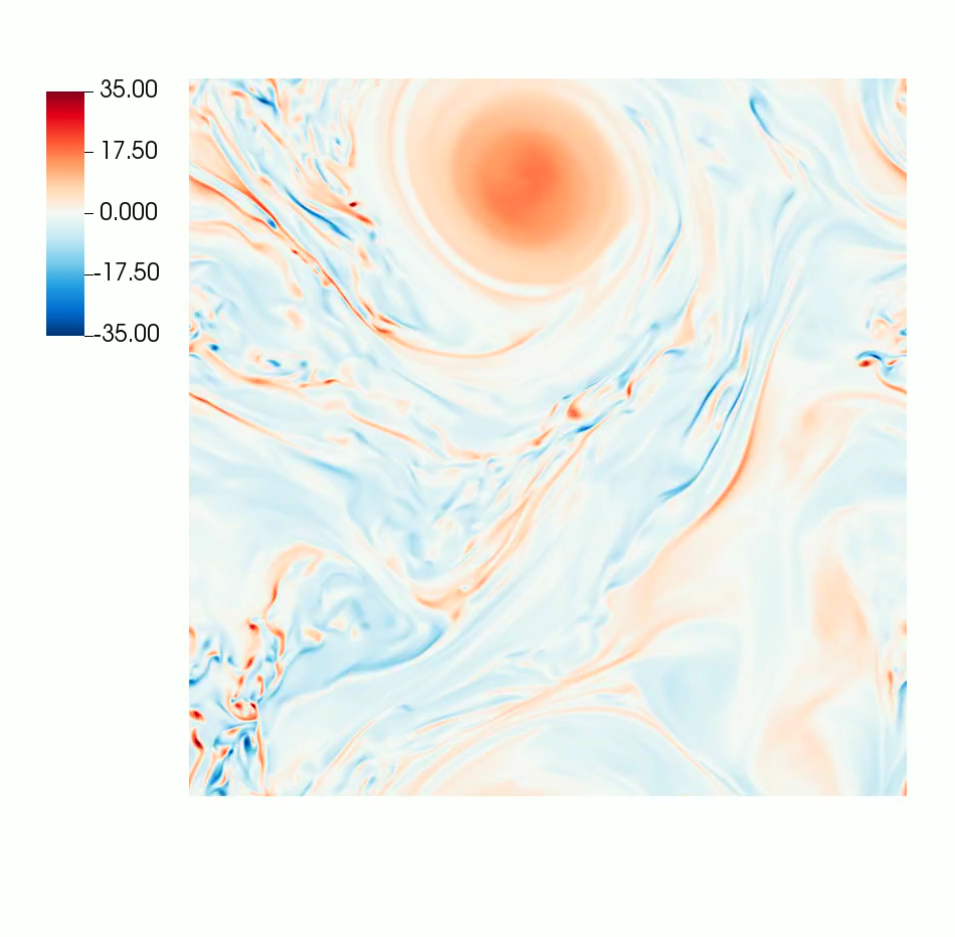
\includegraphics[width=.8\textwidth]{images/SC_Om2B30_XY.png}}{images/Om2B30_XY.mp4}

        %\includegraphics[width=\textwidth]{files/XYB100ux.png}
        %\includegraphics[width=\textwidth]{files/XZB100ux.png}
        %\includegraphics[width = \textwidth]{files/B100Spec.pdf}
    \emp
    \bmp{.33}
        \centering
        $1/Ro = 1$
        \vspace{2pt}
        \embedvideo*{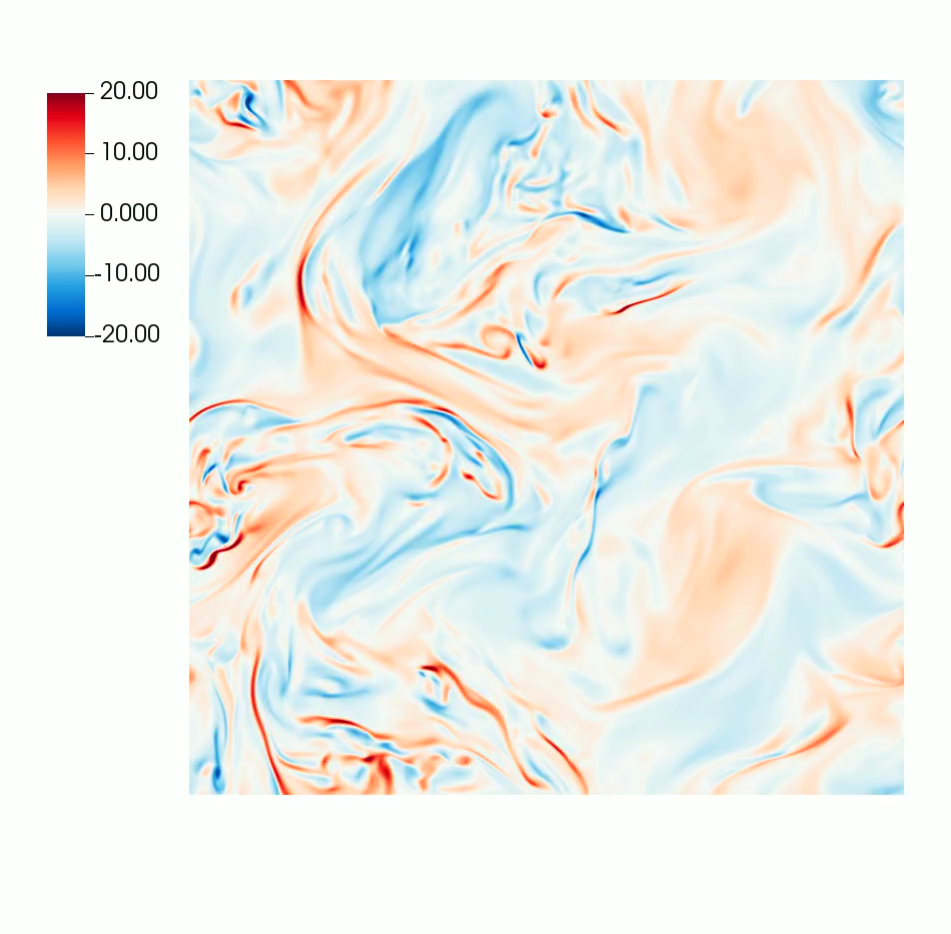
\includegraphics[width=.8\textwidth]{images/SC_Om1B30_XY.png}}{images/Om1B30_XY.mp4}
        \vspace{5pt}
        $1/Ro = 5$
        \vspace{2pt}
        \embedvideo*{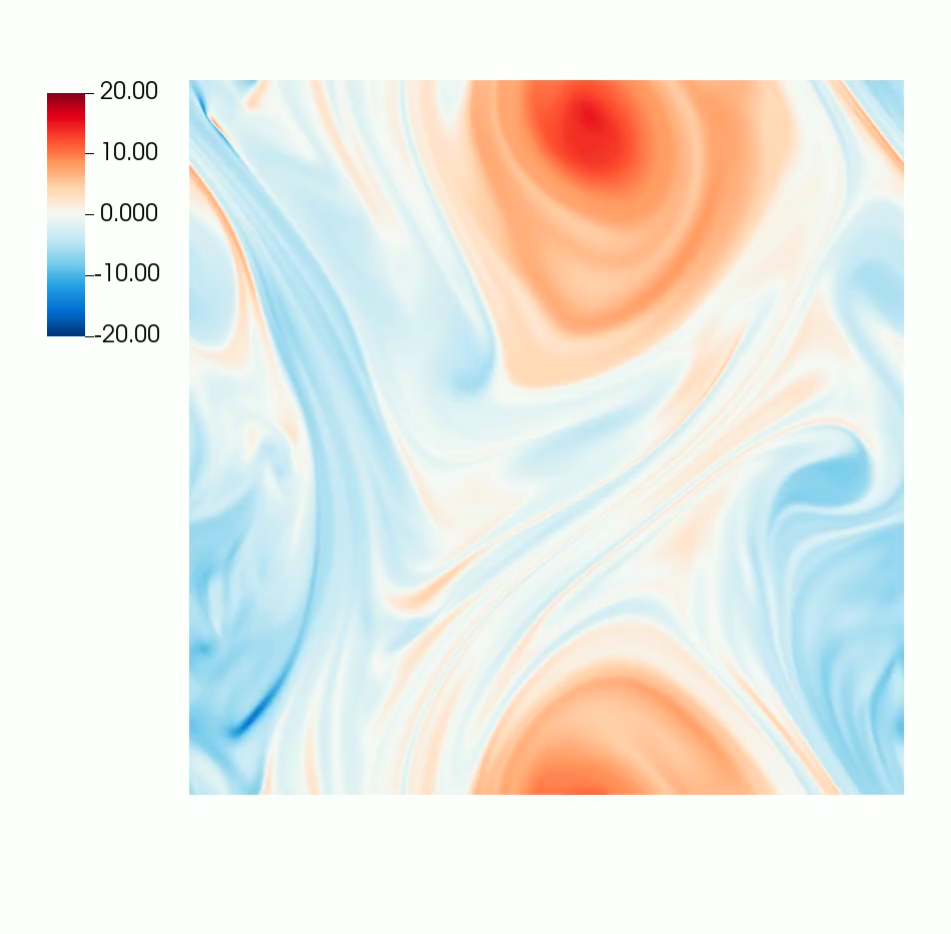
\includegraphics[width=.8\textwidth]{images/SC_Om5B30_XY.png}}{images/Om5B30_XY.mp4}

    \emp

\end{frame}

\begin{frame}{Vertically-Invariant Structures in the flow}
    \centering
    \bmp{0.07}
        $\omega_z$
    \emp
    \bmp{0.31}
        \centering
        $1/Ro = 1$
        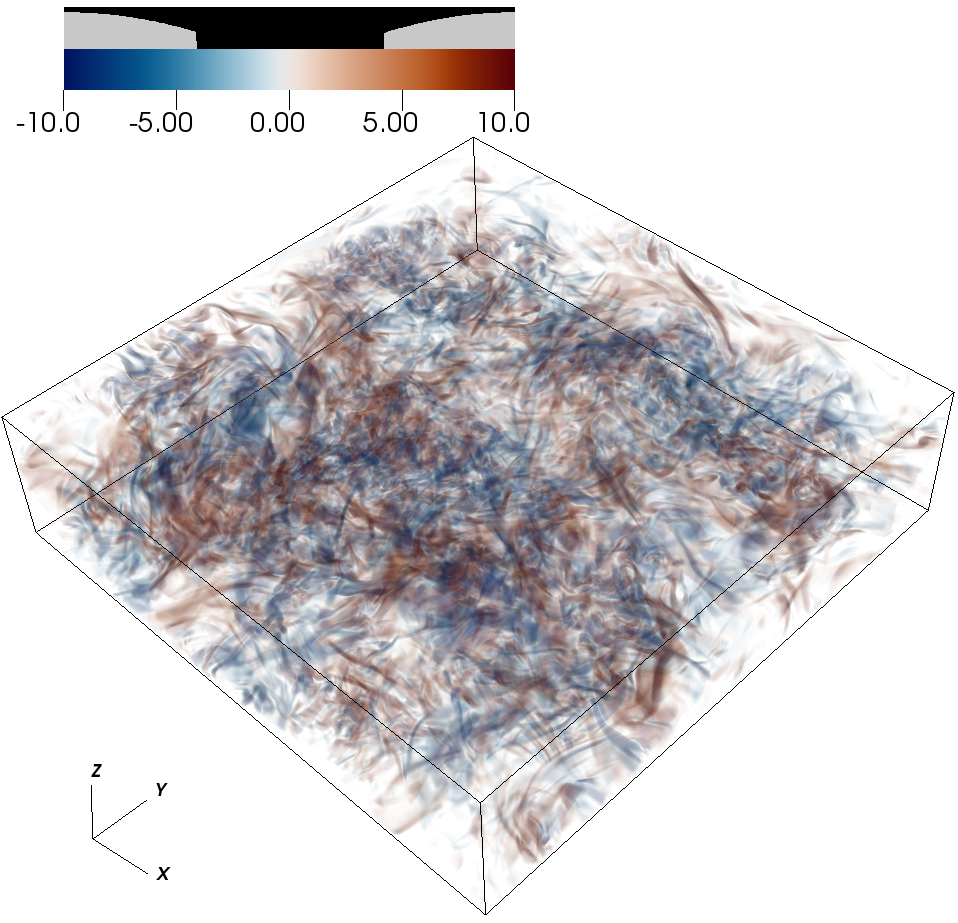
\includegraphics[width=.95\textwidth]{images/vortz_Om0.5_vr2.png}
    \emp
    \bmp{0.31}
        \centering
        $1/Ro = 2$
        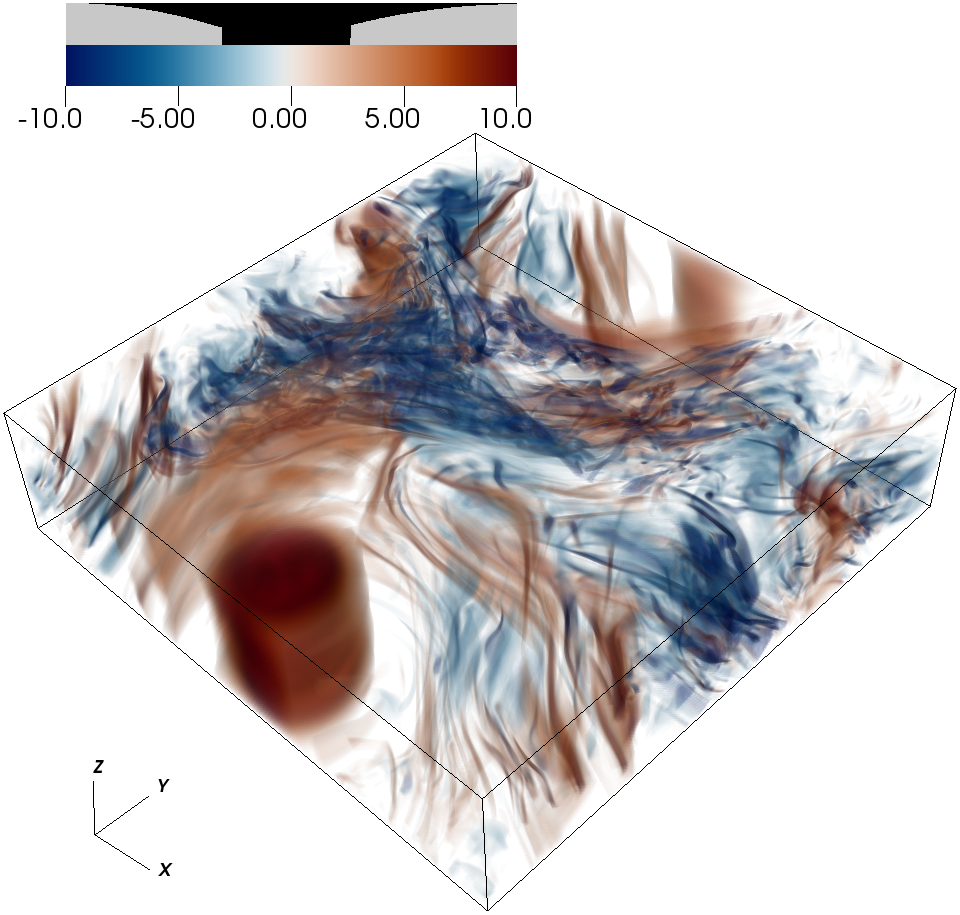
\includegraphics[width=.95\textwidth]{images/vortz_Om2_vr2.png}
    \emp
    \bmp{0.31}
        \centering
        $1/Ro = 10$
        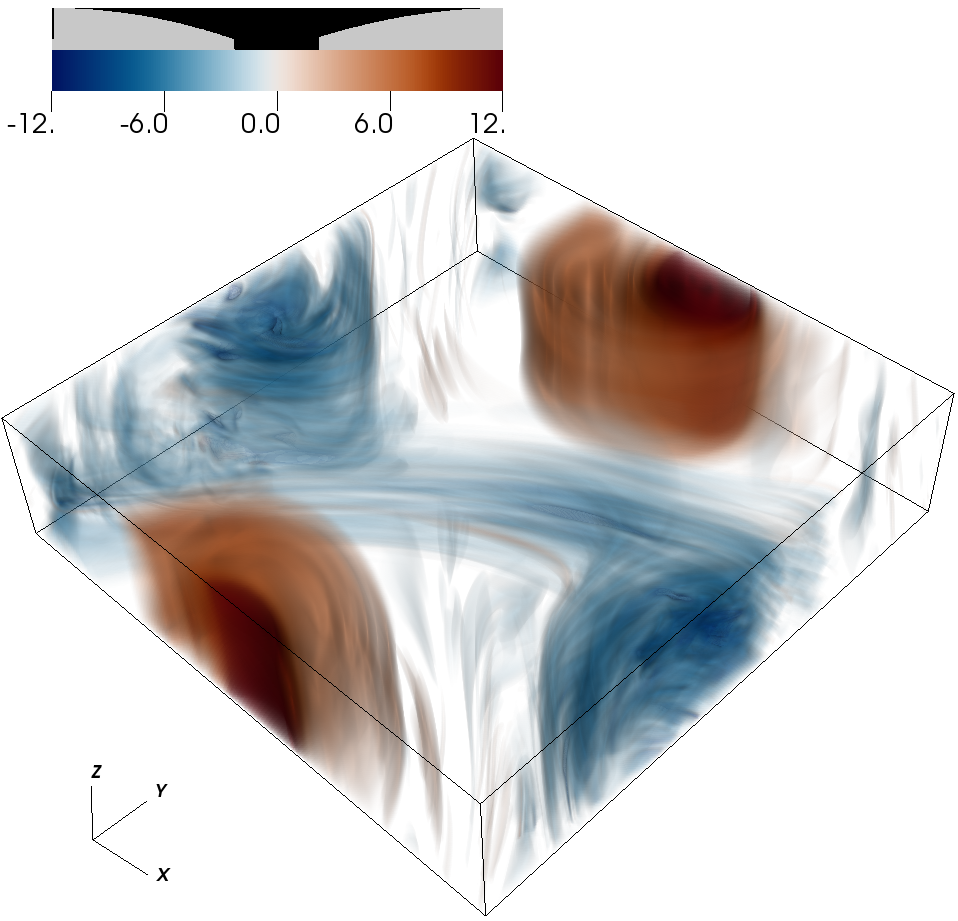
\includegraphics[width=.95\textwidth]{images/vortz_Om10_vr2.png}
    \emp
\end{frame}


% Energy Spectrum
\begin{frame}{Inverse Energy Cascade}

    \bmp{.46}
        \centering
        {\small Nonrotating}
        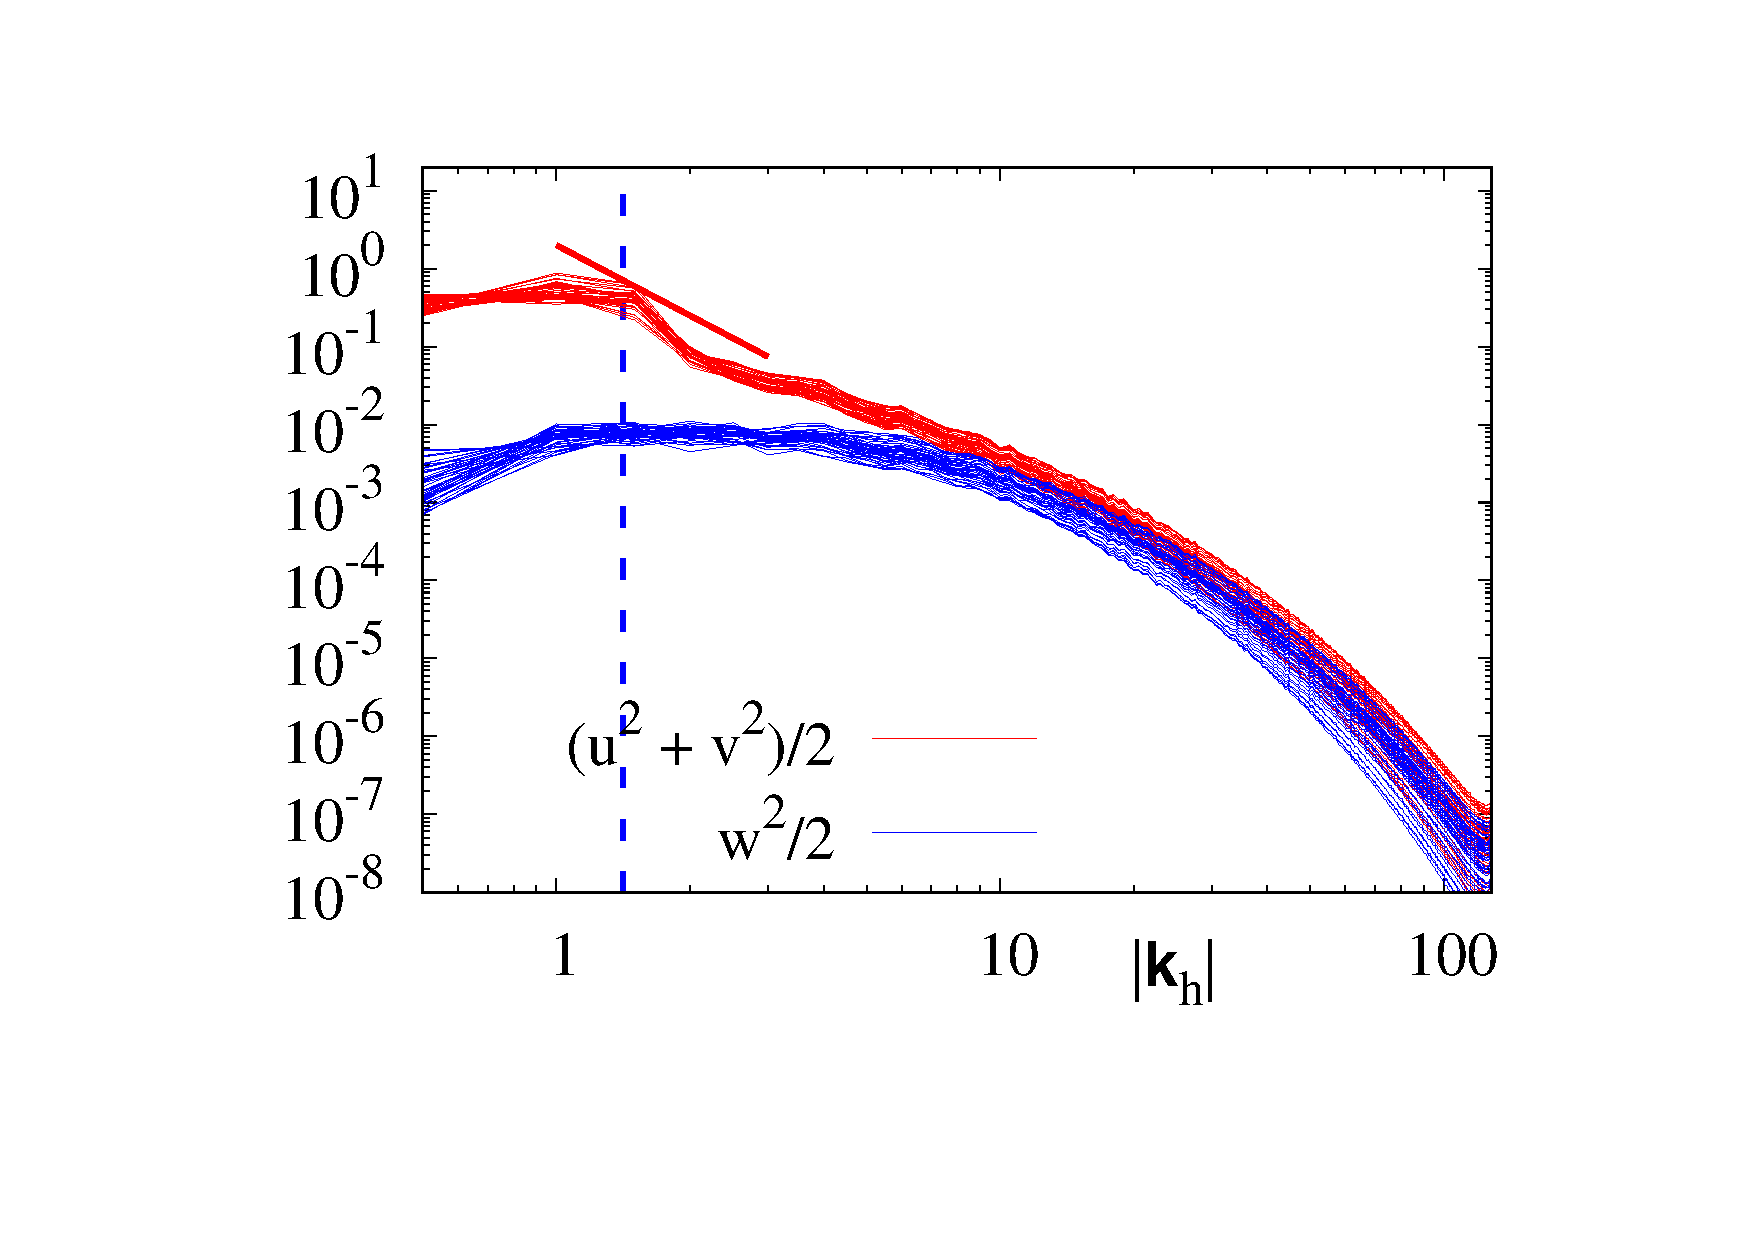
\includegraphics[width=.91\textwidth]{images/B30Spec.pdf}
    \emp
    \bmp{.46}
        \centering
        {\small $Ro^{-1} = 1$}
        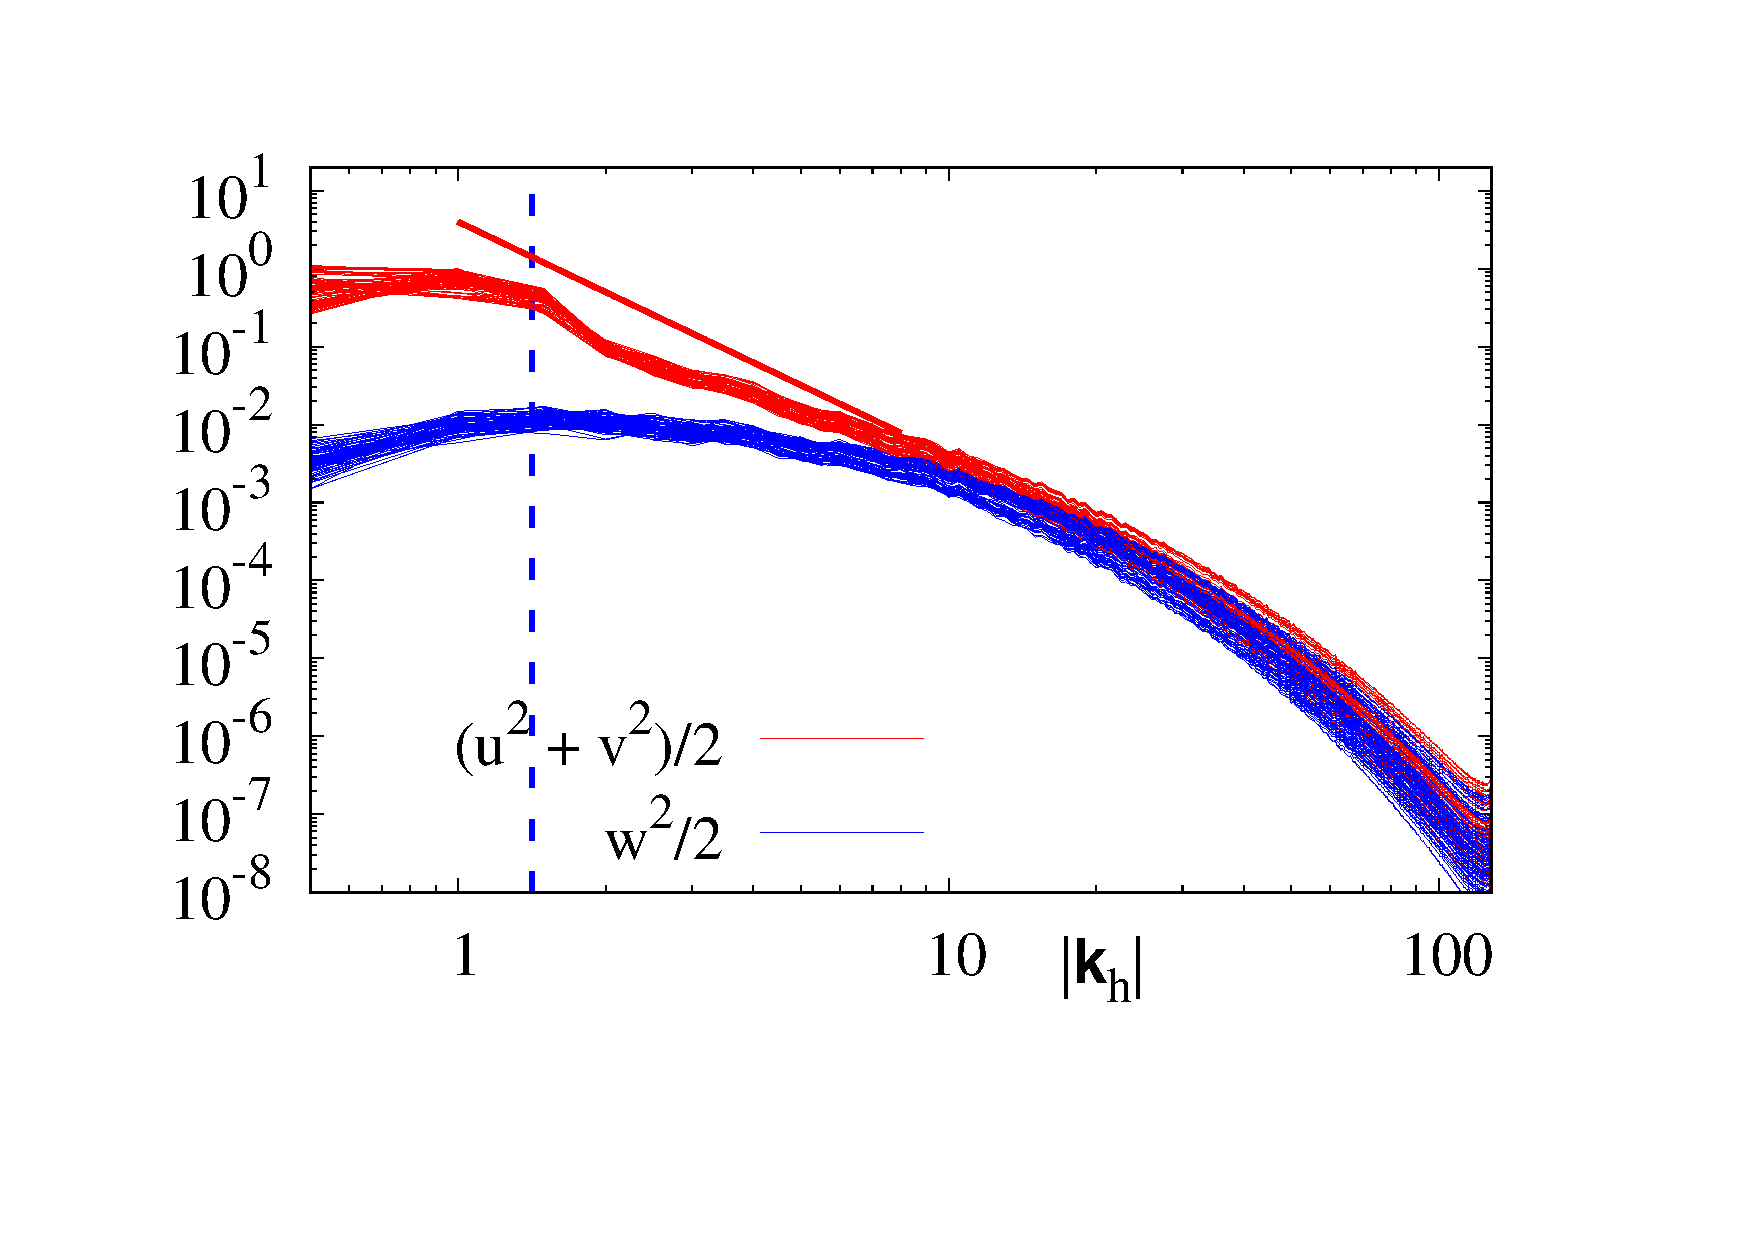
\includegraphics[width=.99\textwidth]{images/Om1Spec.pdf}
    \emp

    \bmp{.46}
        \centering
        {\small $Ro^{-1} = 2$}
        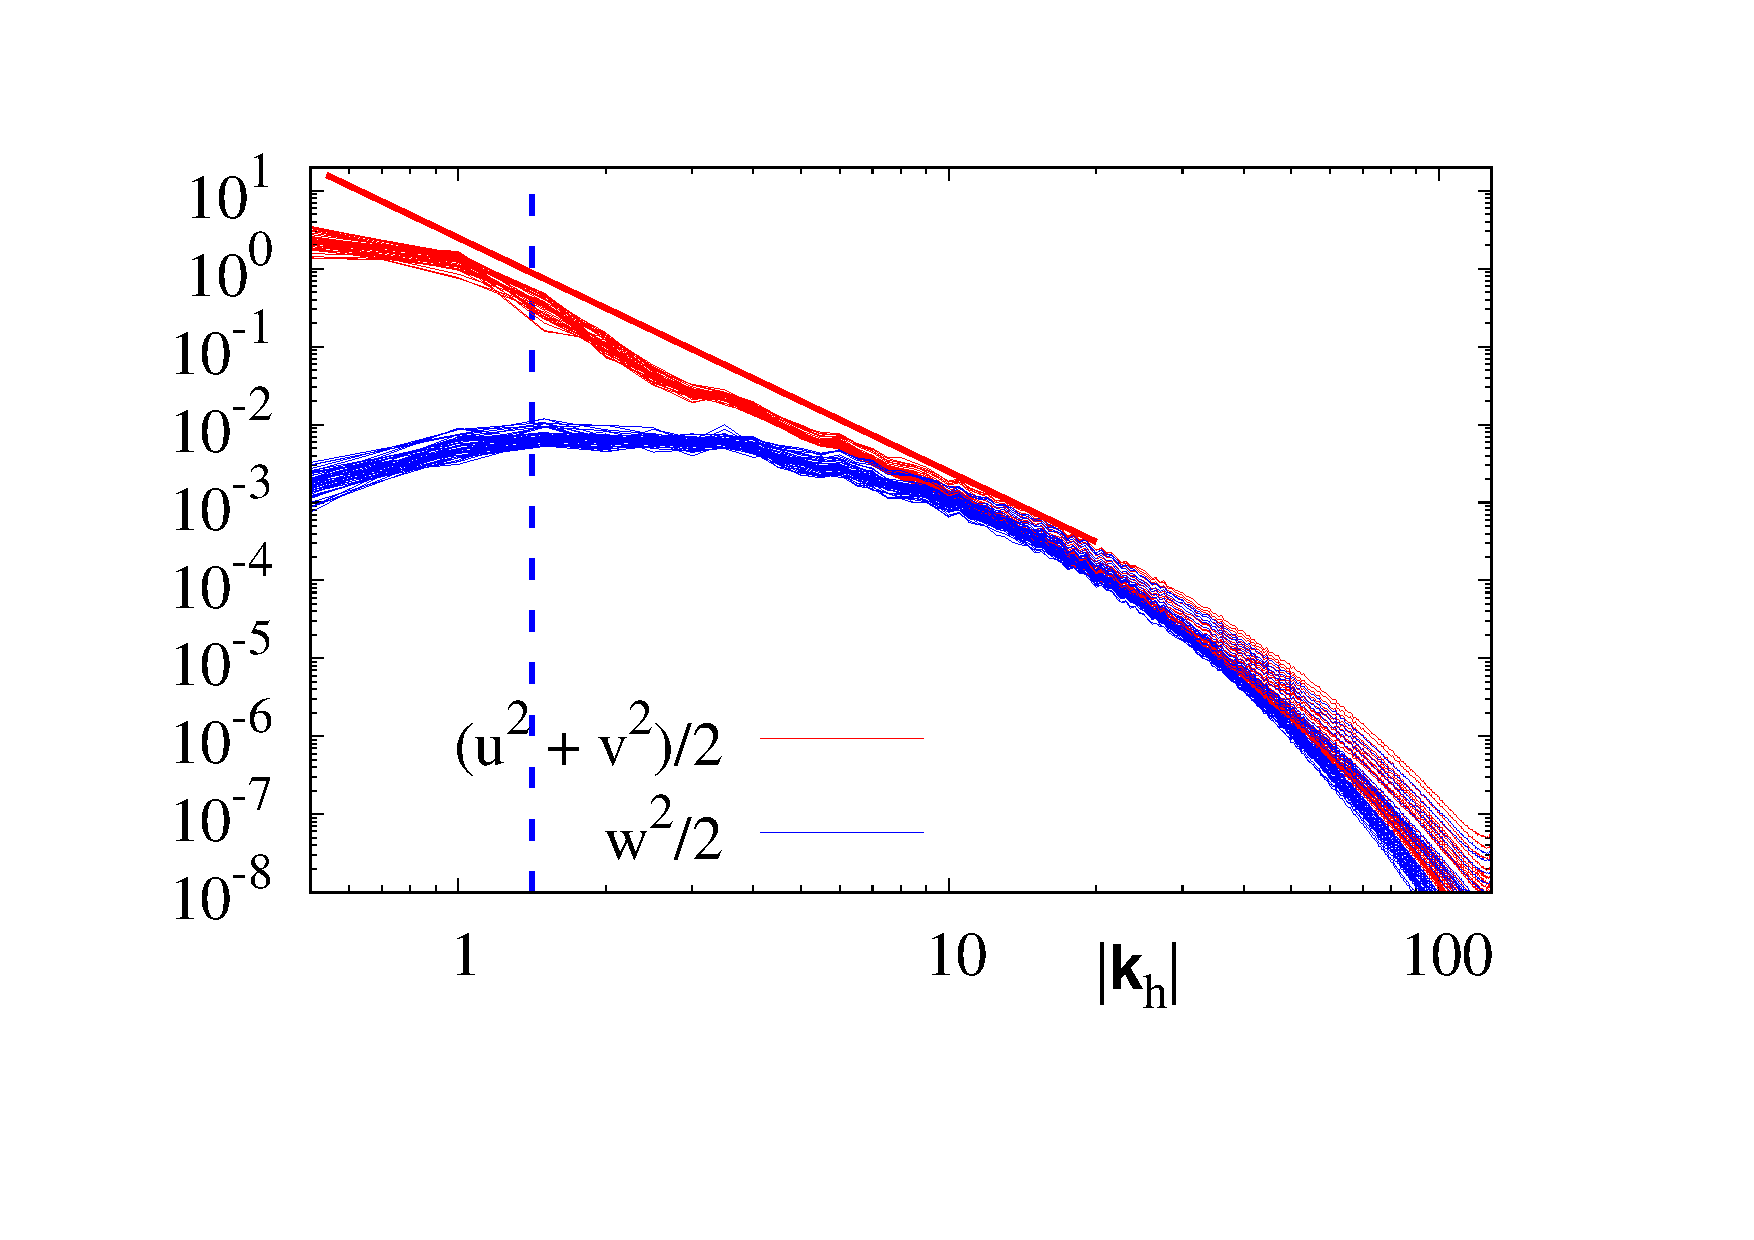
\includegraphics[width=.94\textwidth]{images/Om2Spec.pdf}
    \emp
    \bmp{.46}
        \centering
        {\small $Ro^{-1} = 5$}
        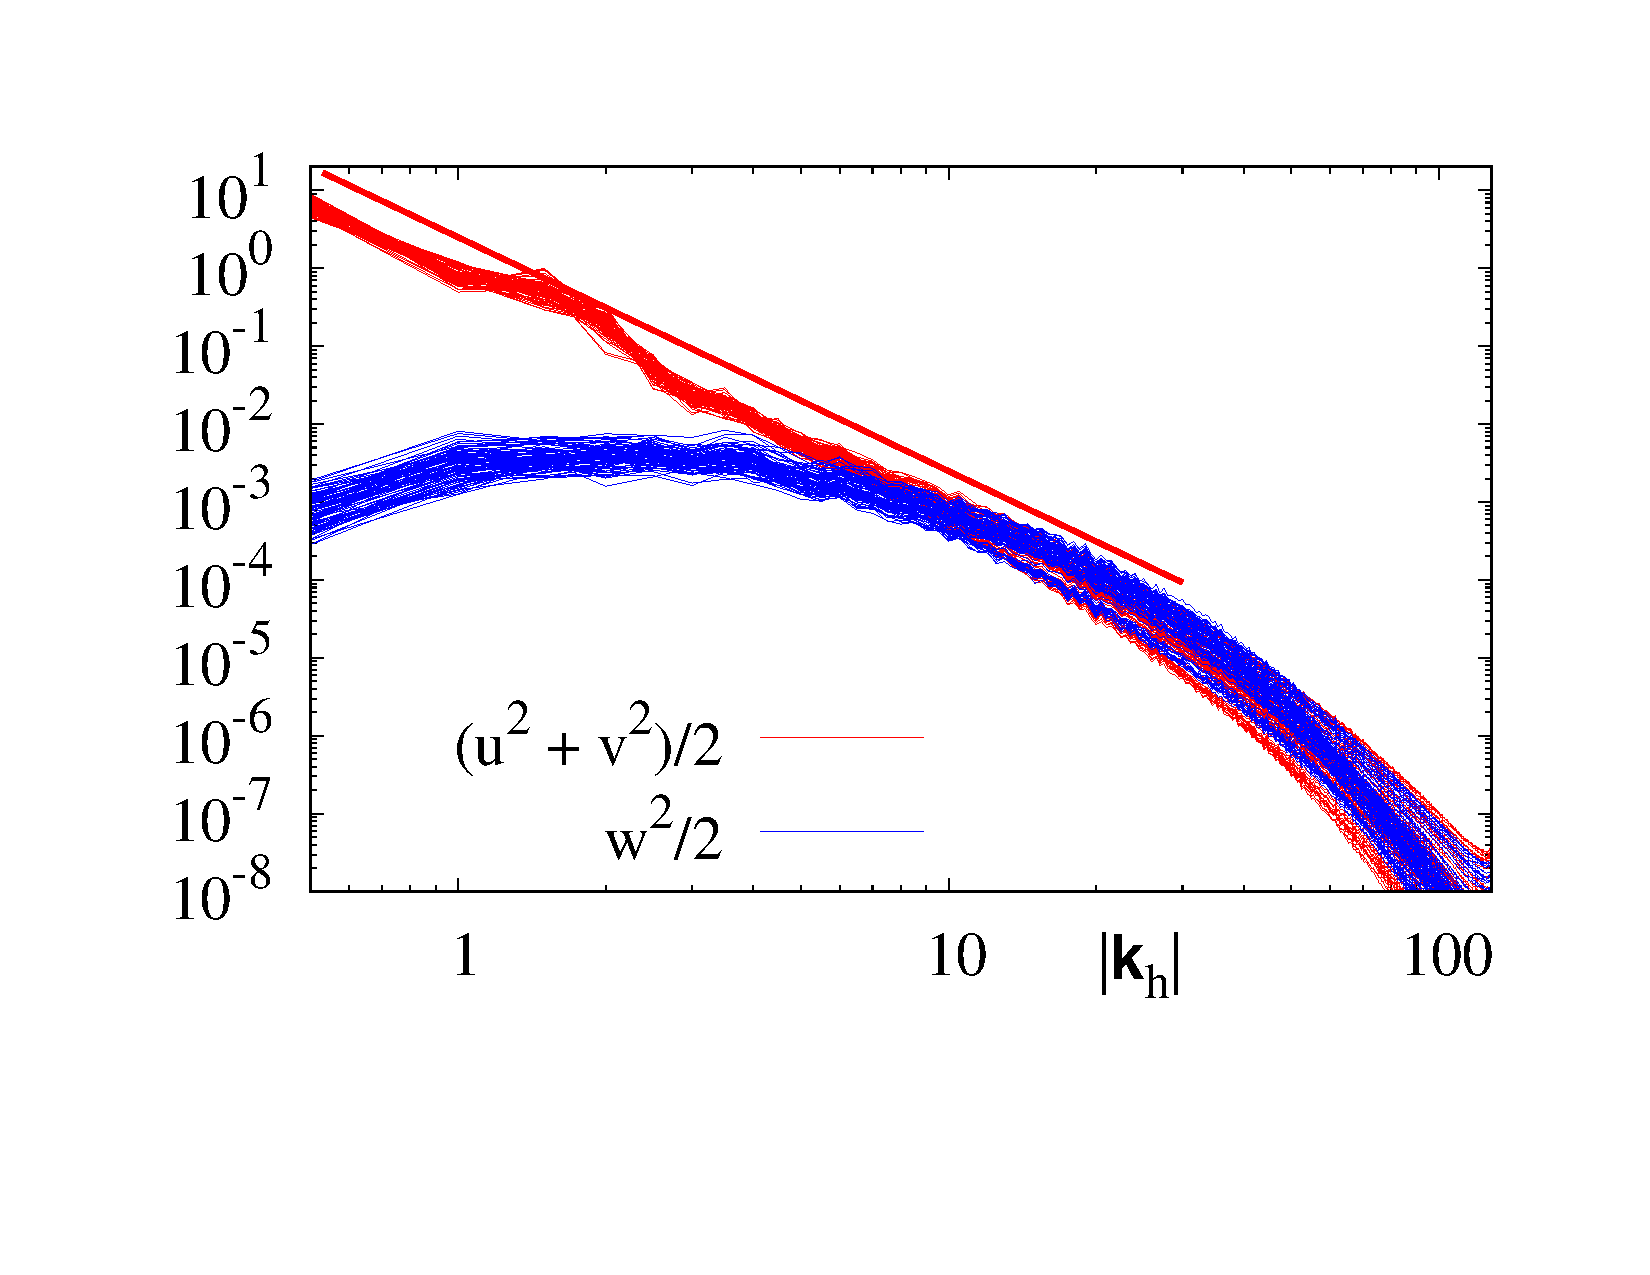
\includegraphics[width=.96\textwidth]{images/Om5Spec.pdf}
    \emp

\end{frame}
%RMS Data
\begin{frame}{R.M.S. Data}
    \bmp{.49}
        \centering
        %u_h 
        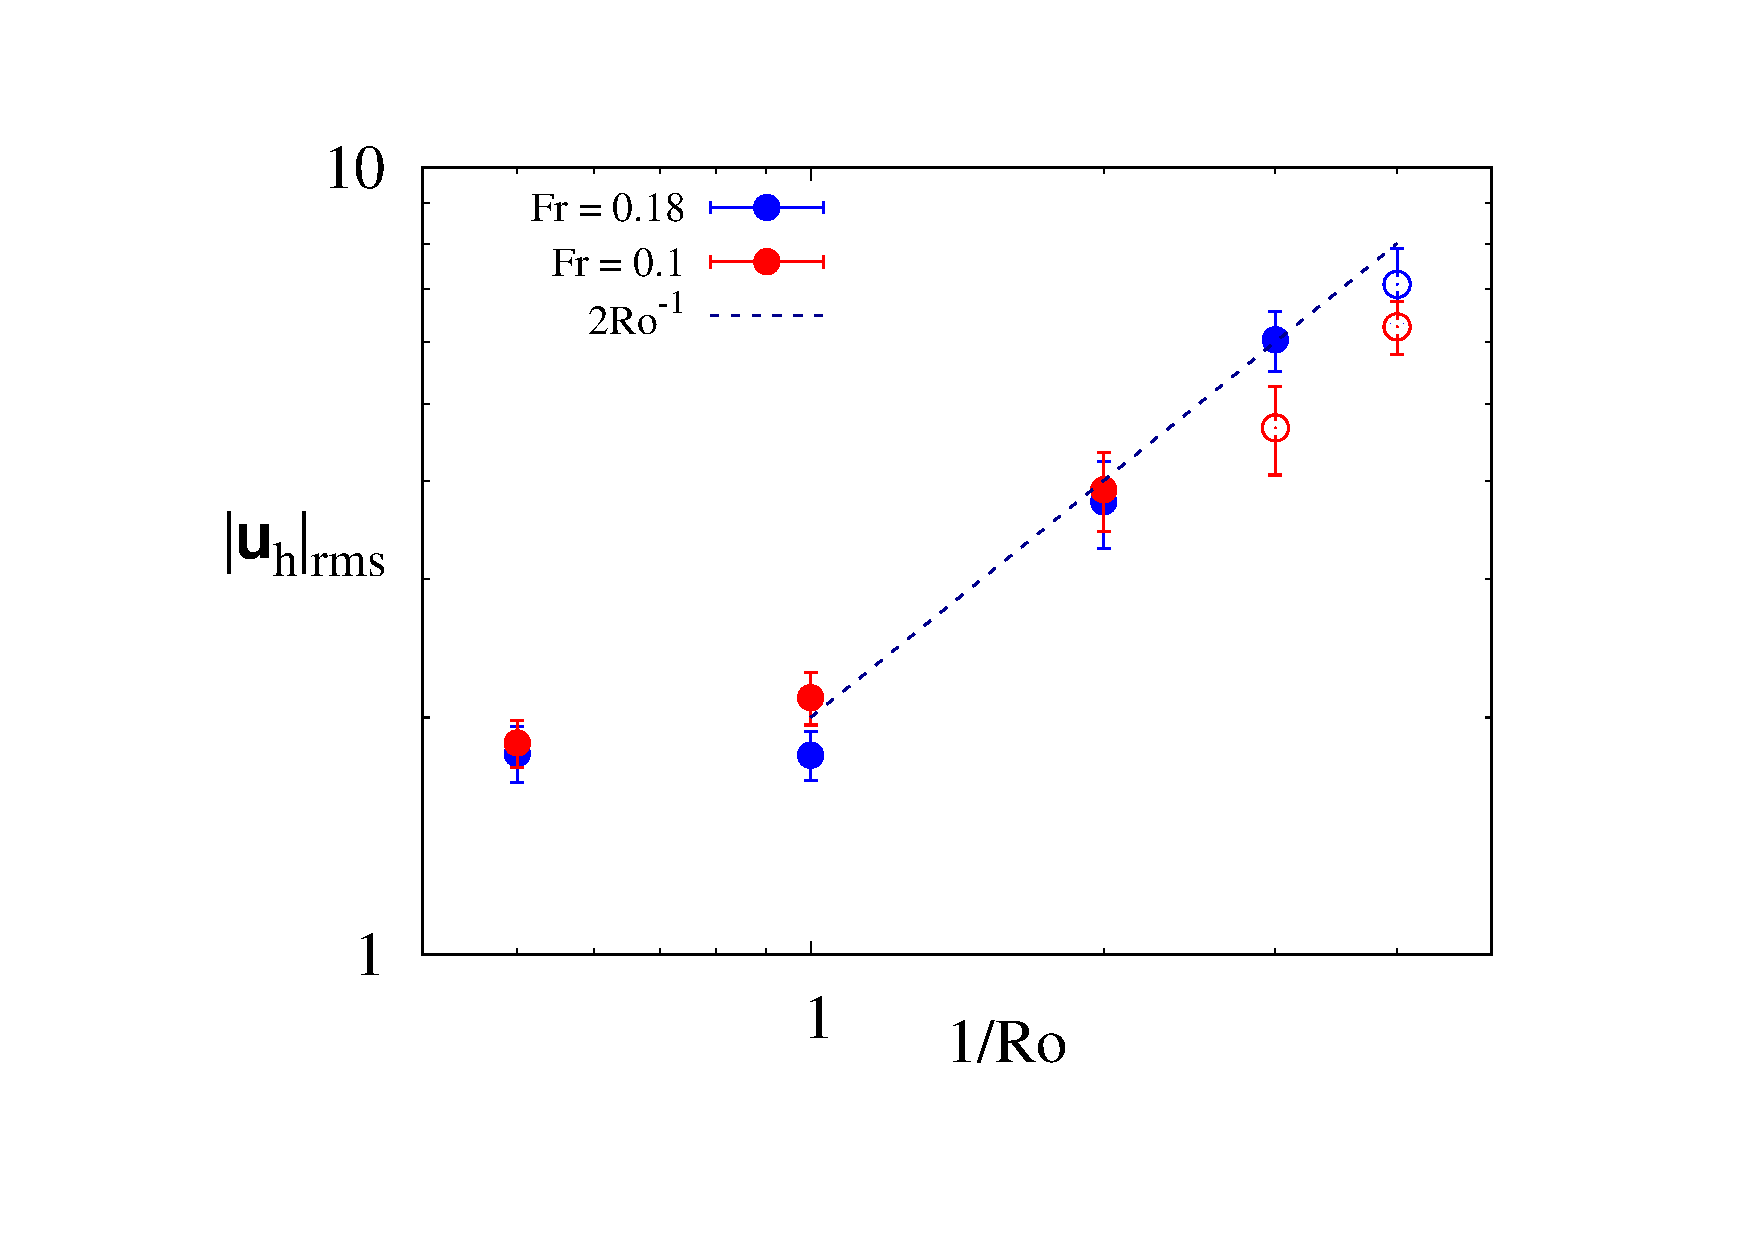
\includegraphics[width=1\textwidth]{images/urms_plot.pdf}
    \emp
    \bmp{.49}
        % w
        \centering
        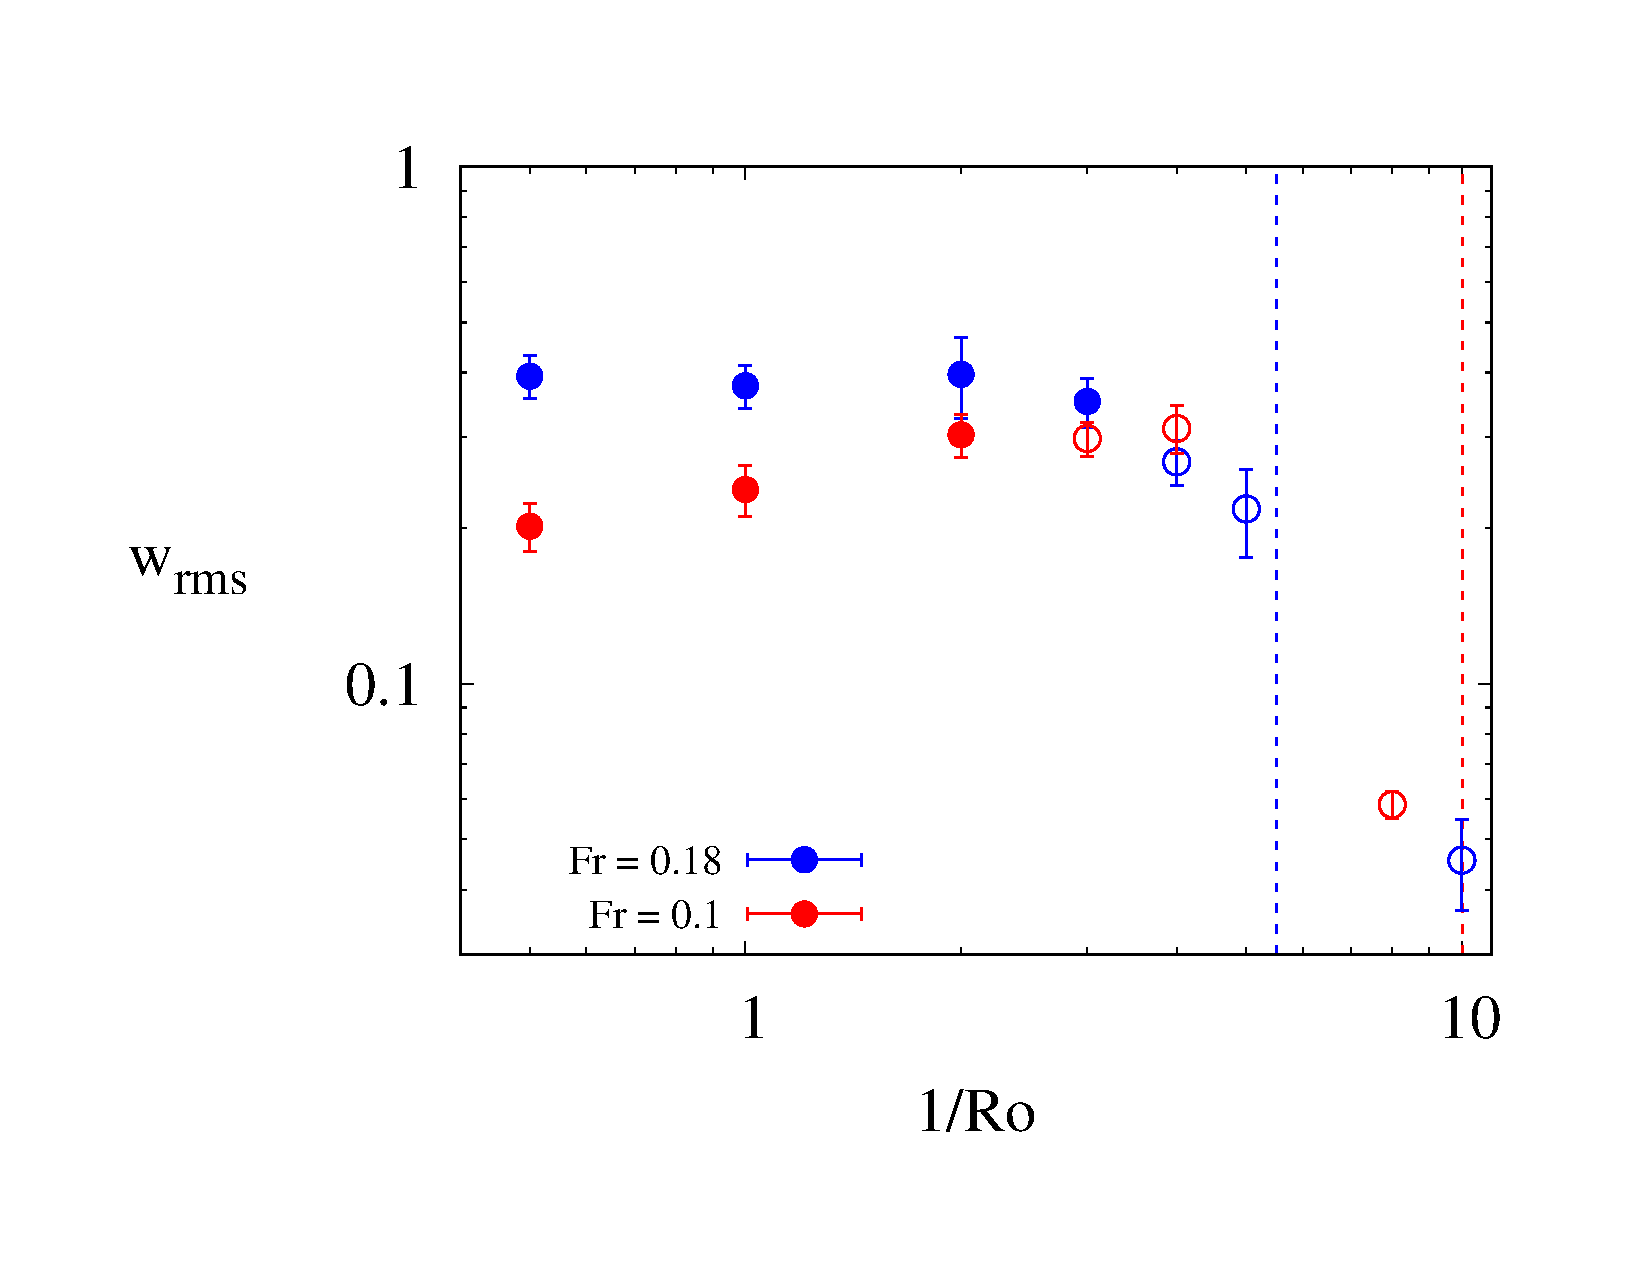
\includegraphics[width=.96\textwidth]{images/wrms_plot.pdf}
    \emp
    
\end{frame}

\begin{frame}{Vertically-Averaged Flow: $\quad \widehat{(\cdot)} \equiv
\frac{1}{L_z}\int(\cdot)dz}
    \centering
    \bmp{.1}
        \centering
        {\footnotesize $\widehat{\omega_z} + Ro^{-1}$}
    \emp
    \bmp{.3}
        \centering
        $1/Ro = 1$
        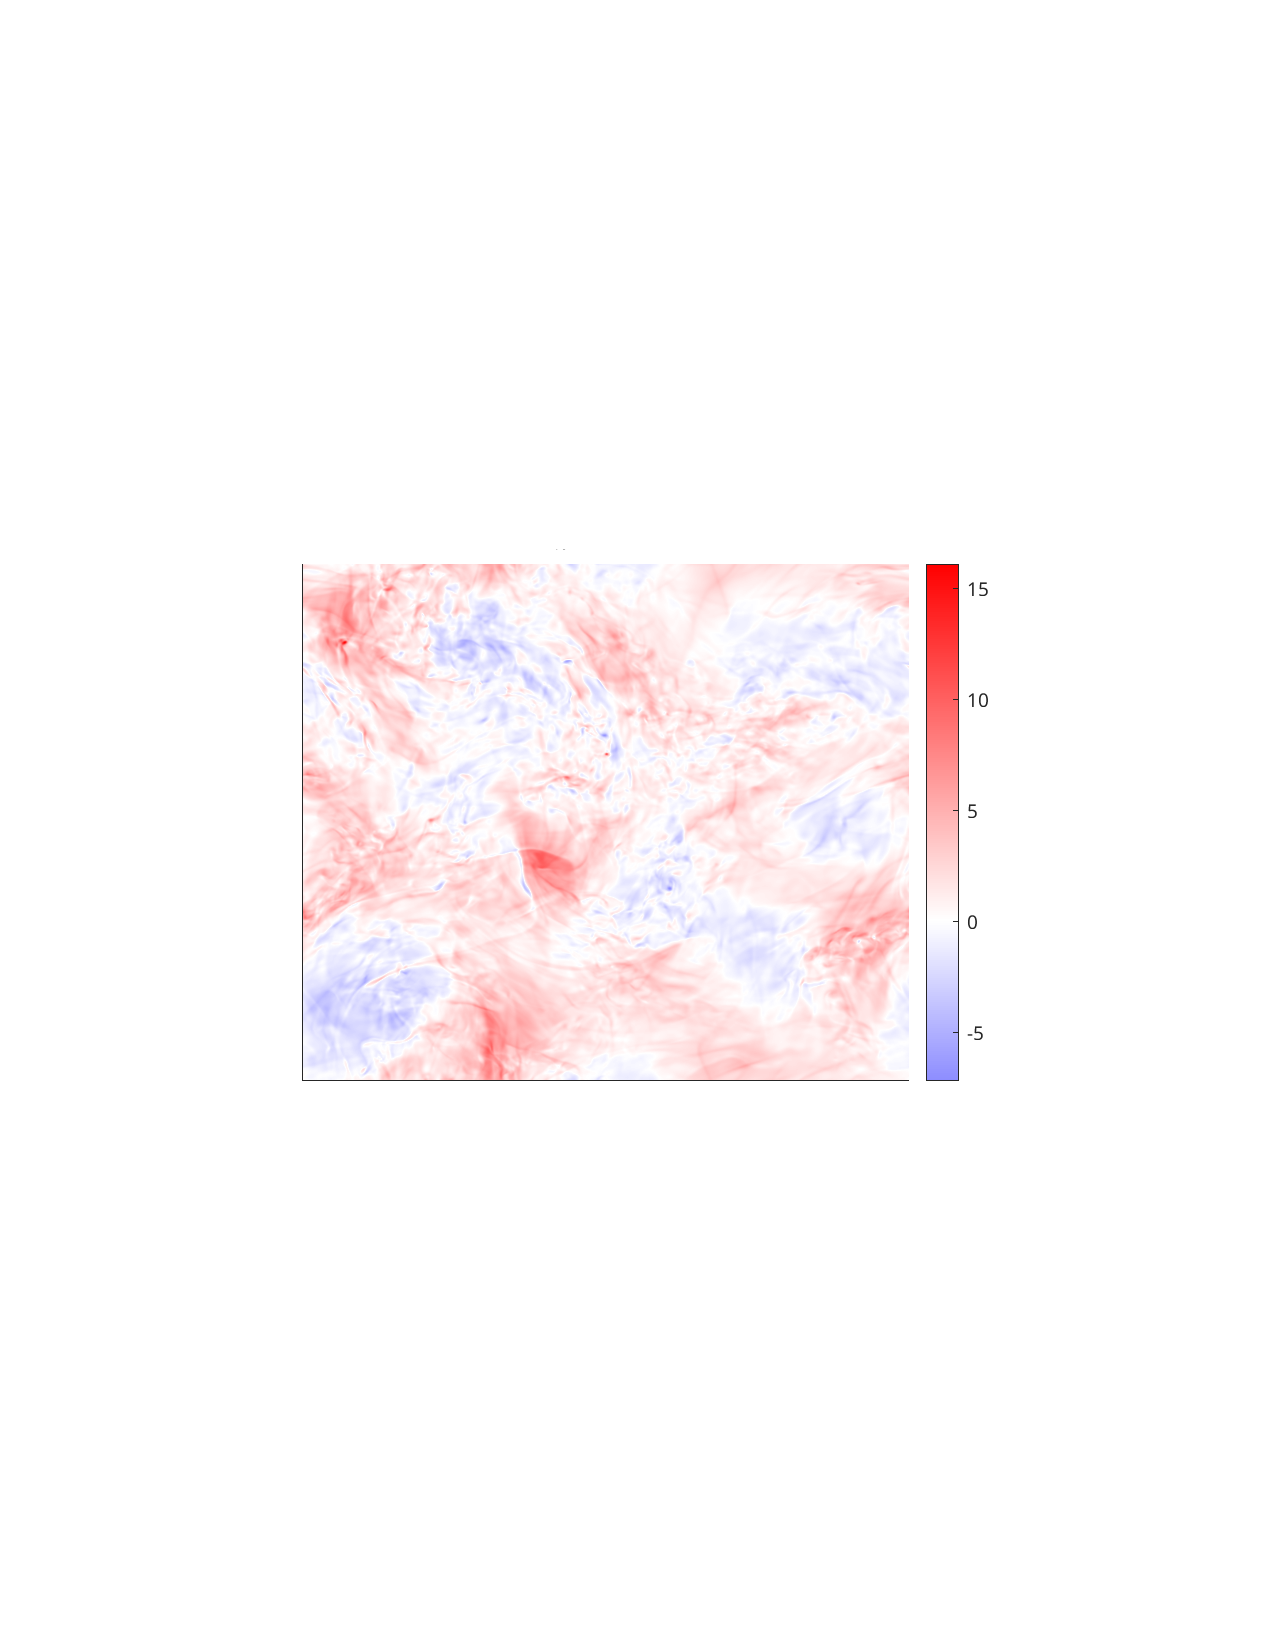
\includegraphics[width=1\textwidth]{images/Om1B30_vortz_bar.pdf}
    \emp
    \bmp{.3}
        \centering
        $1/Ro = 3$
        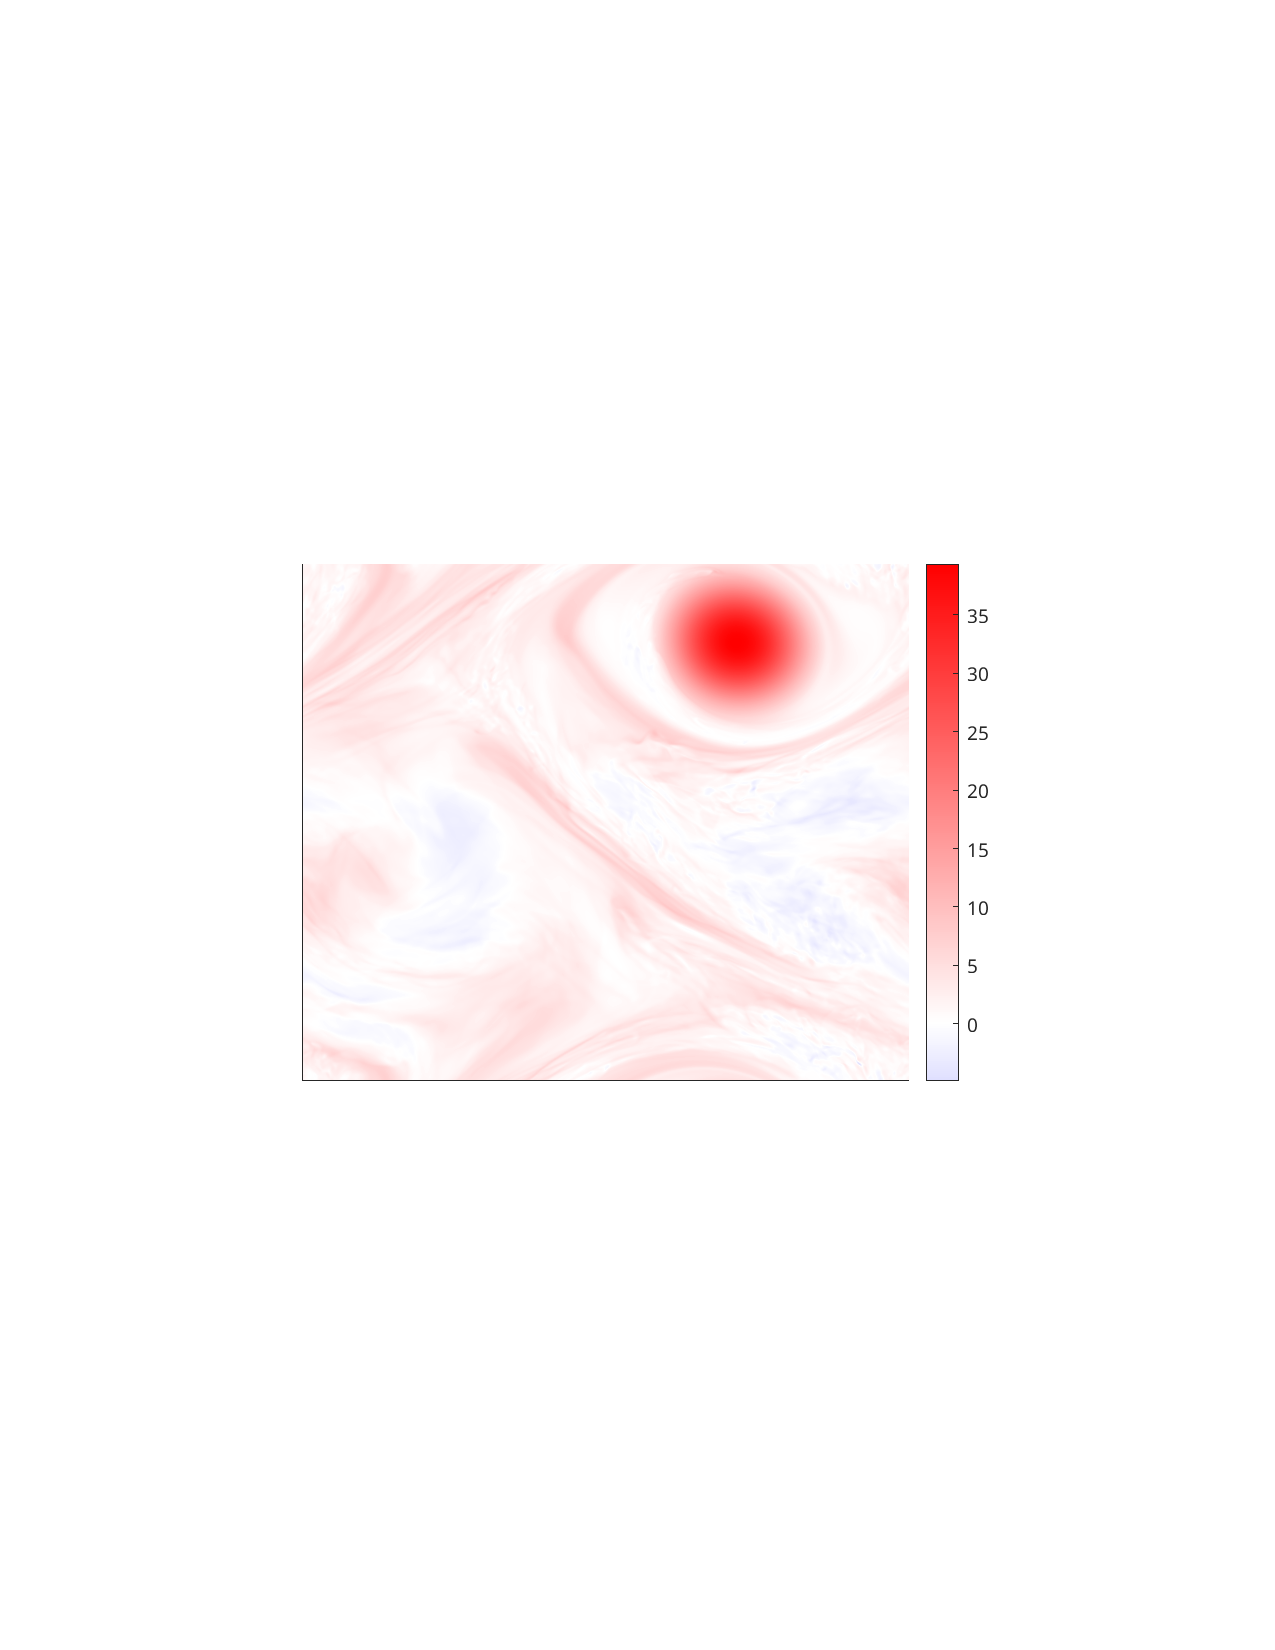
\includegraphics[width=1\textwidth]{images/Om3B30_vortz_bar.pdf}
    \emp
    \bmp{.3}
        \centering
        $1/Ro = 10$
        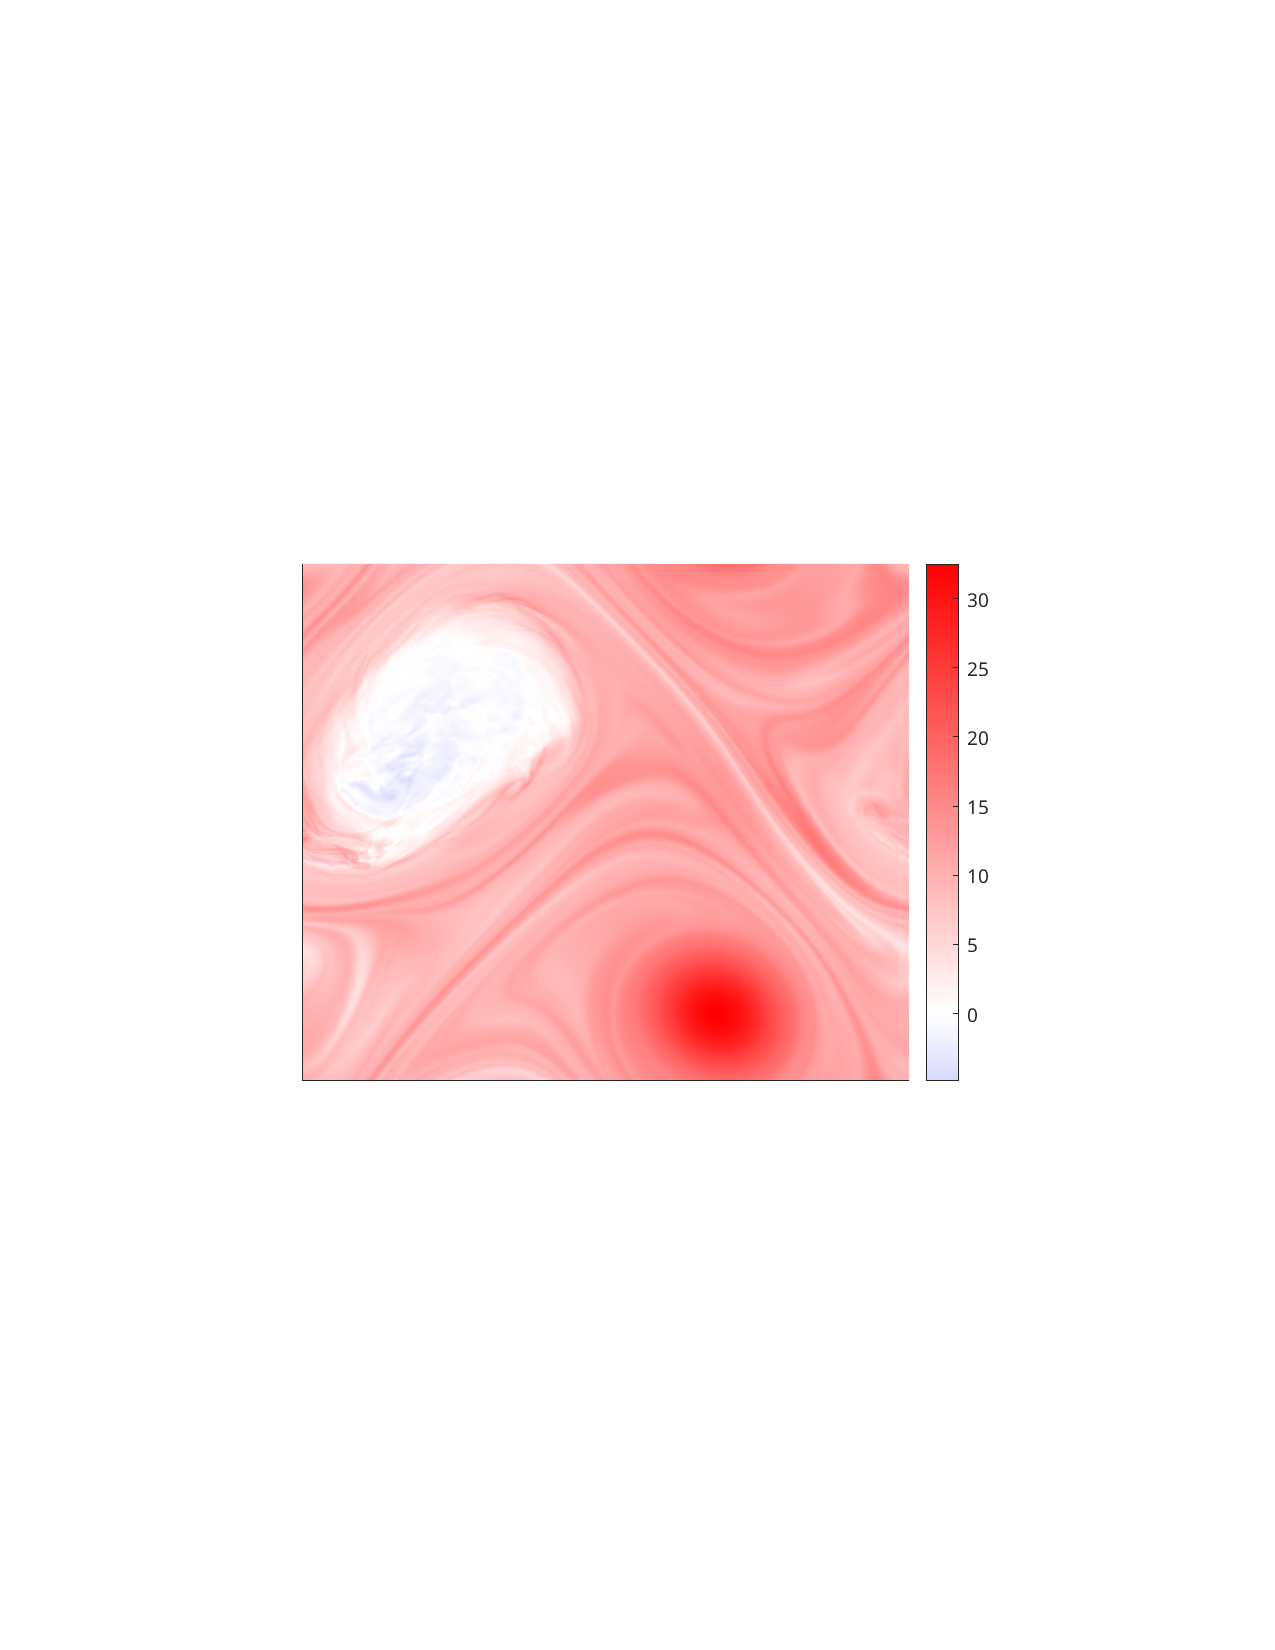
\includegraphics[width=1\textwidth]{images/Om10B30_vortz_bar.pdf}
    \emp

    \bmp{.1}
        \centering
        {\footnotesize $\widehat{w^2}$}
    \emp
    \bmp{.3}
        \centering
        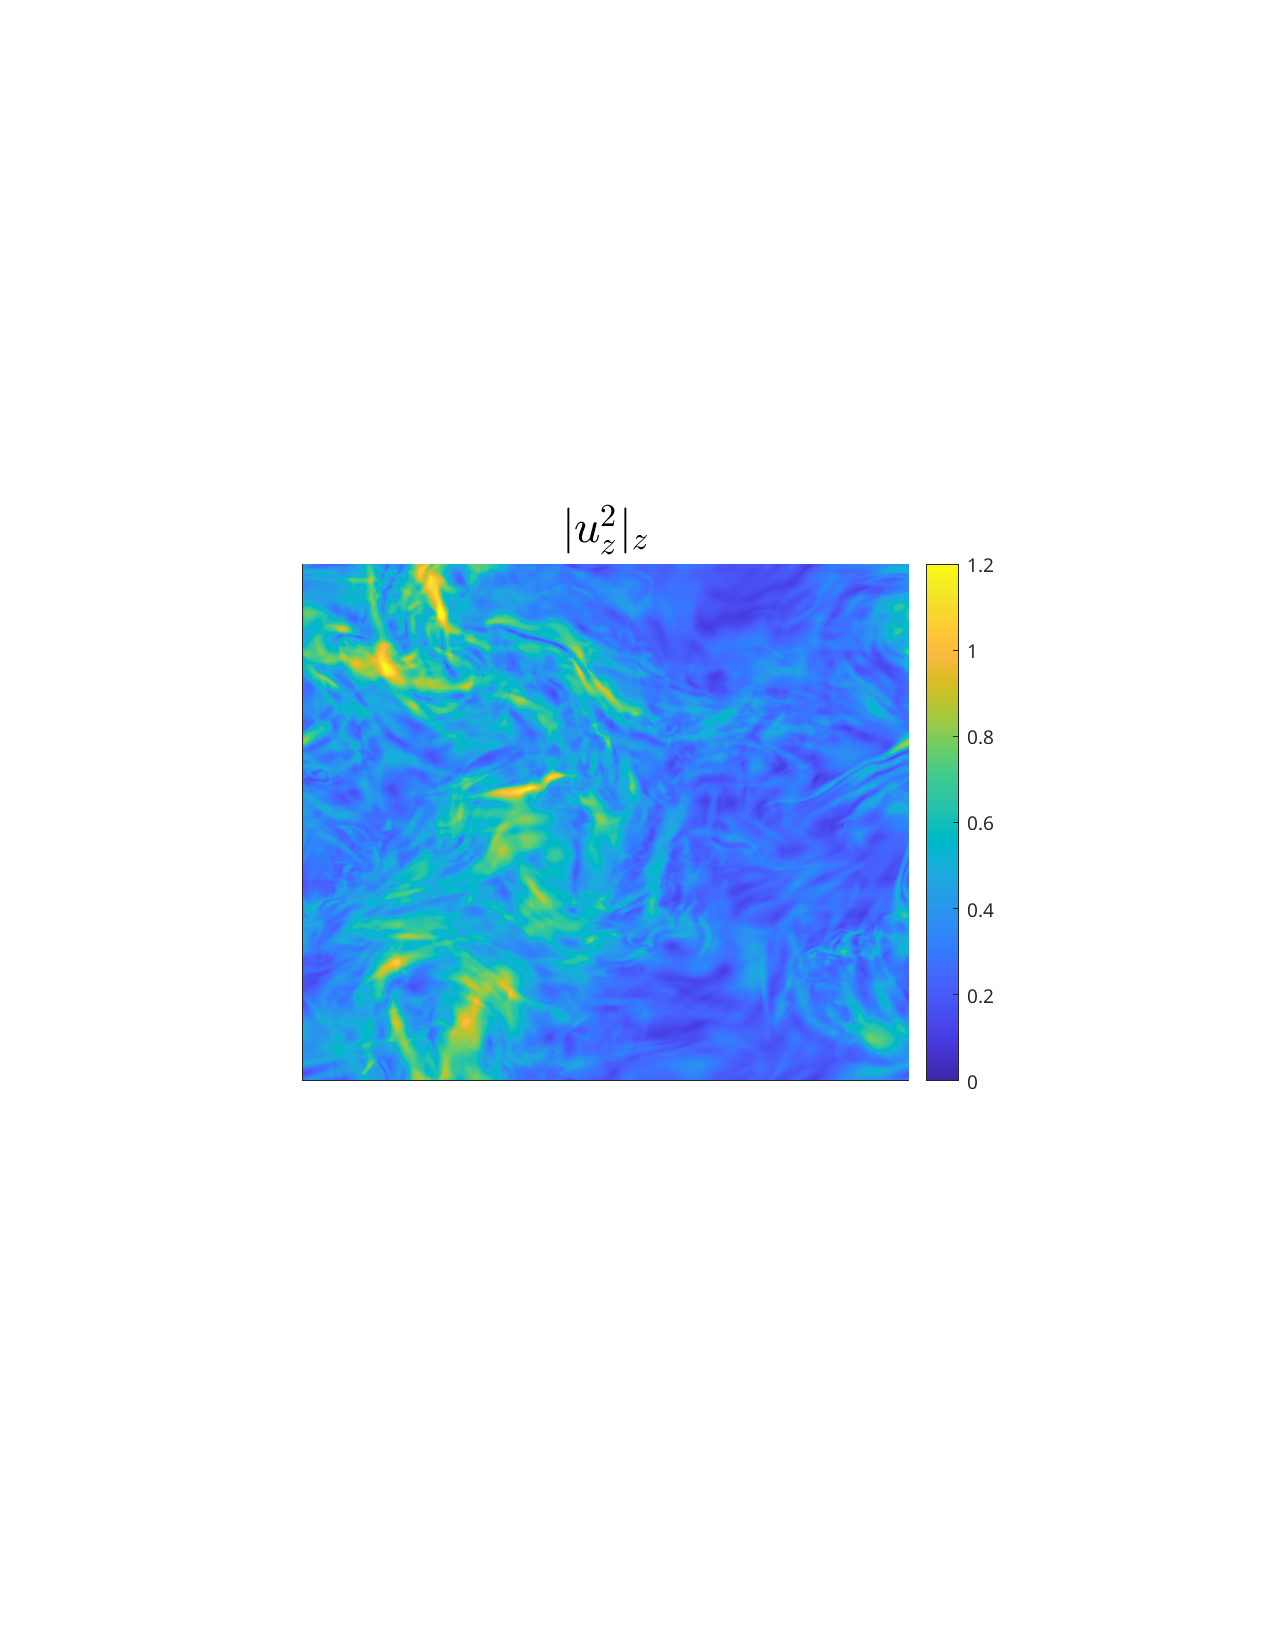
\includegraphics[width=1\textwidth]{images/Om1B30_uzrms_bar.pdf}
    \emp
    \bmp{.3}
        \centering
        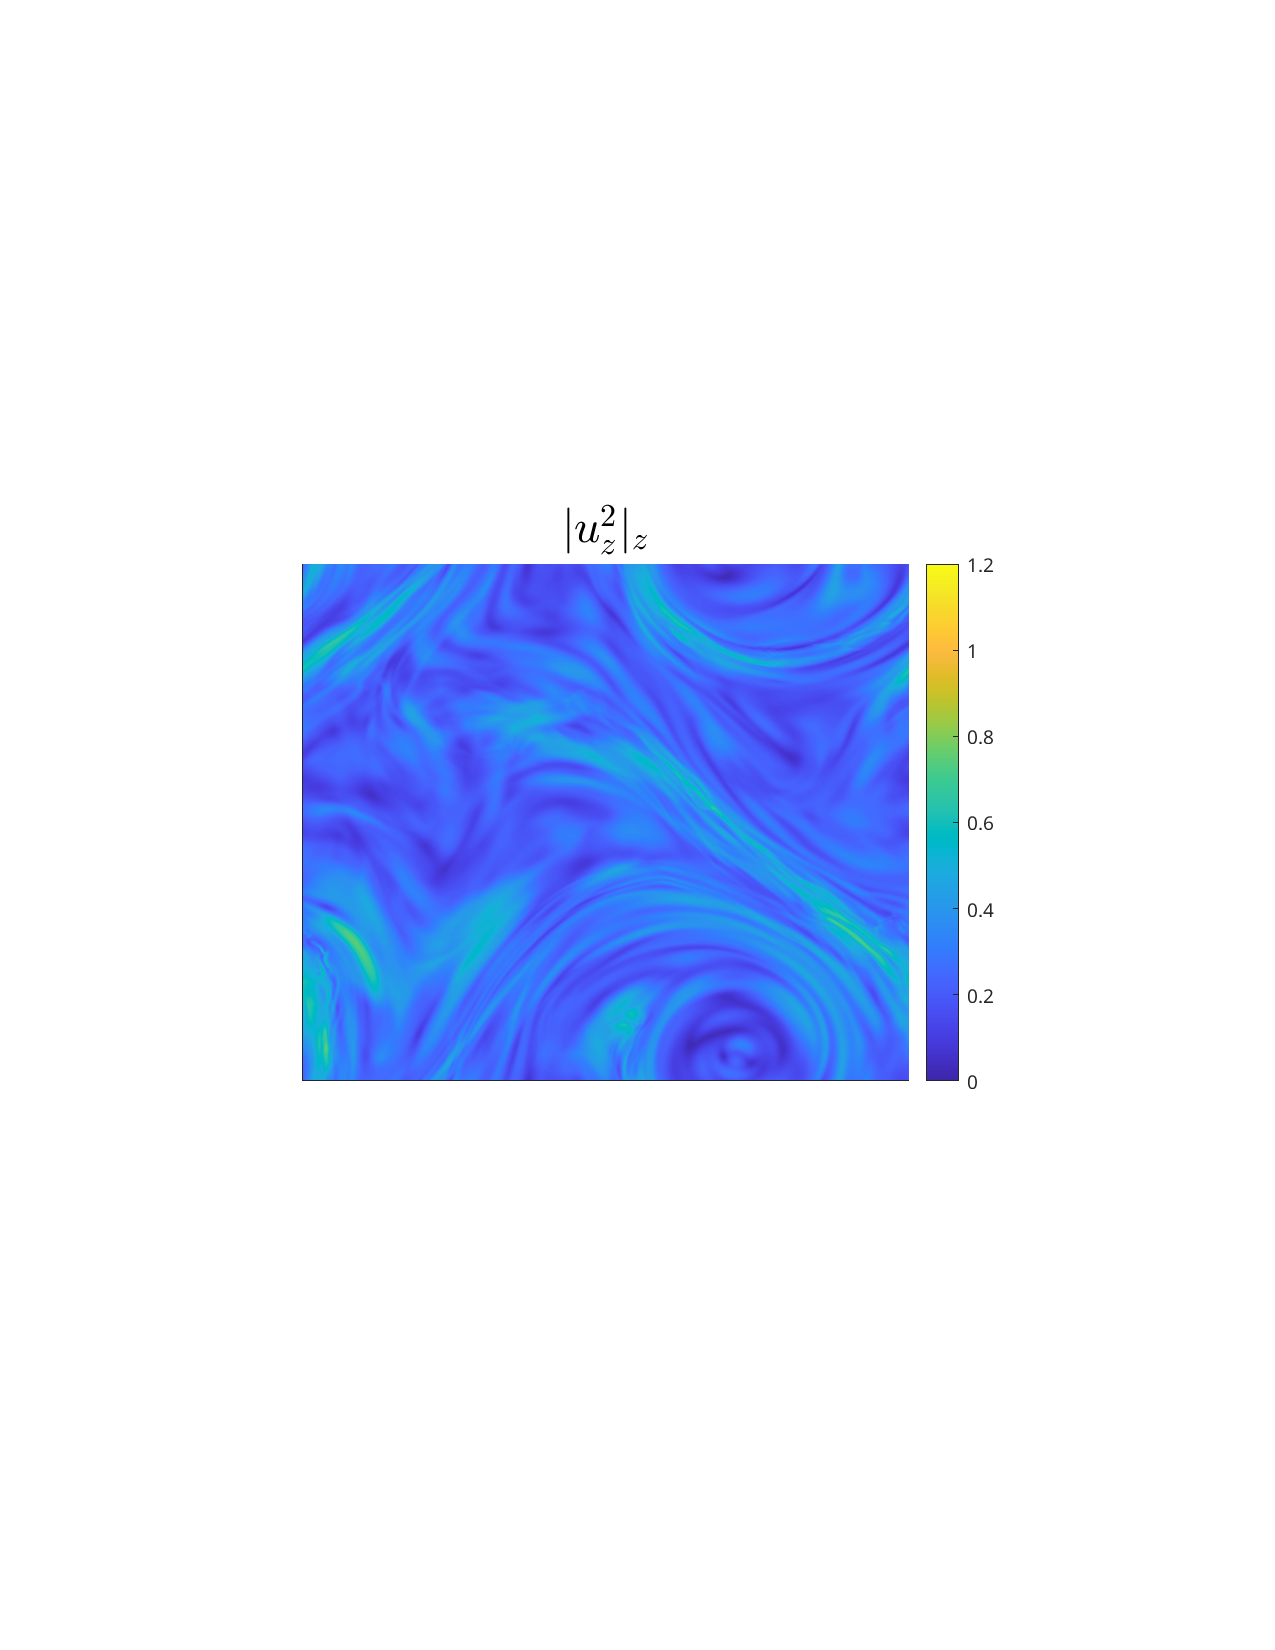
\includegraphics[width=1\textwidth]{images/Om3B30_uzrms_bar.pdf}
    \emp
    \bmp{.3}
        \centering
        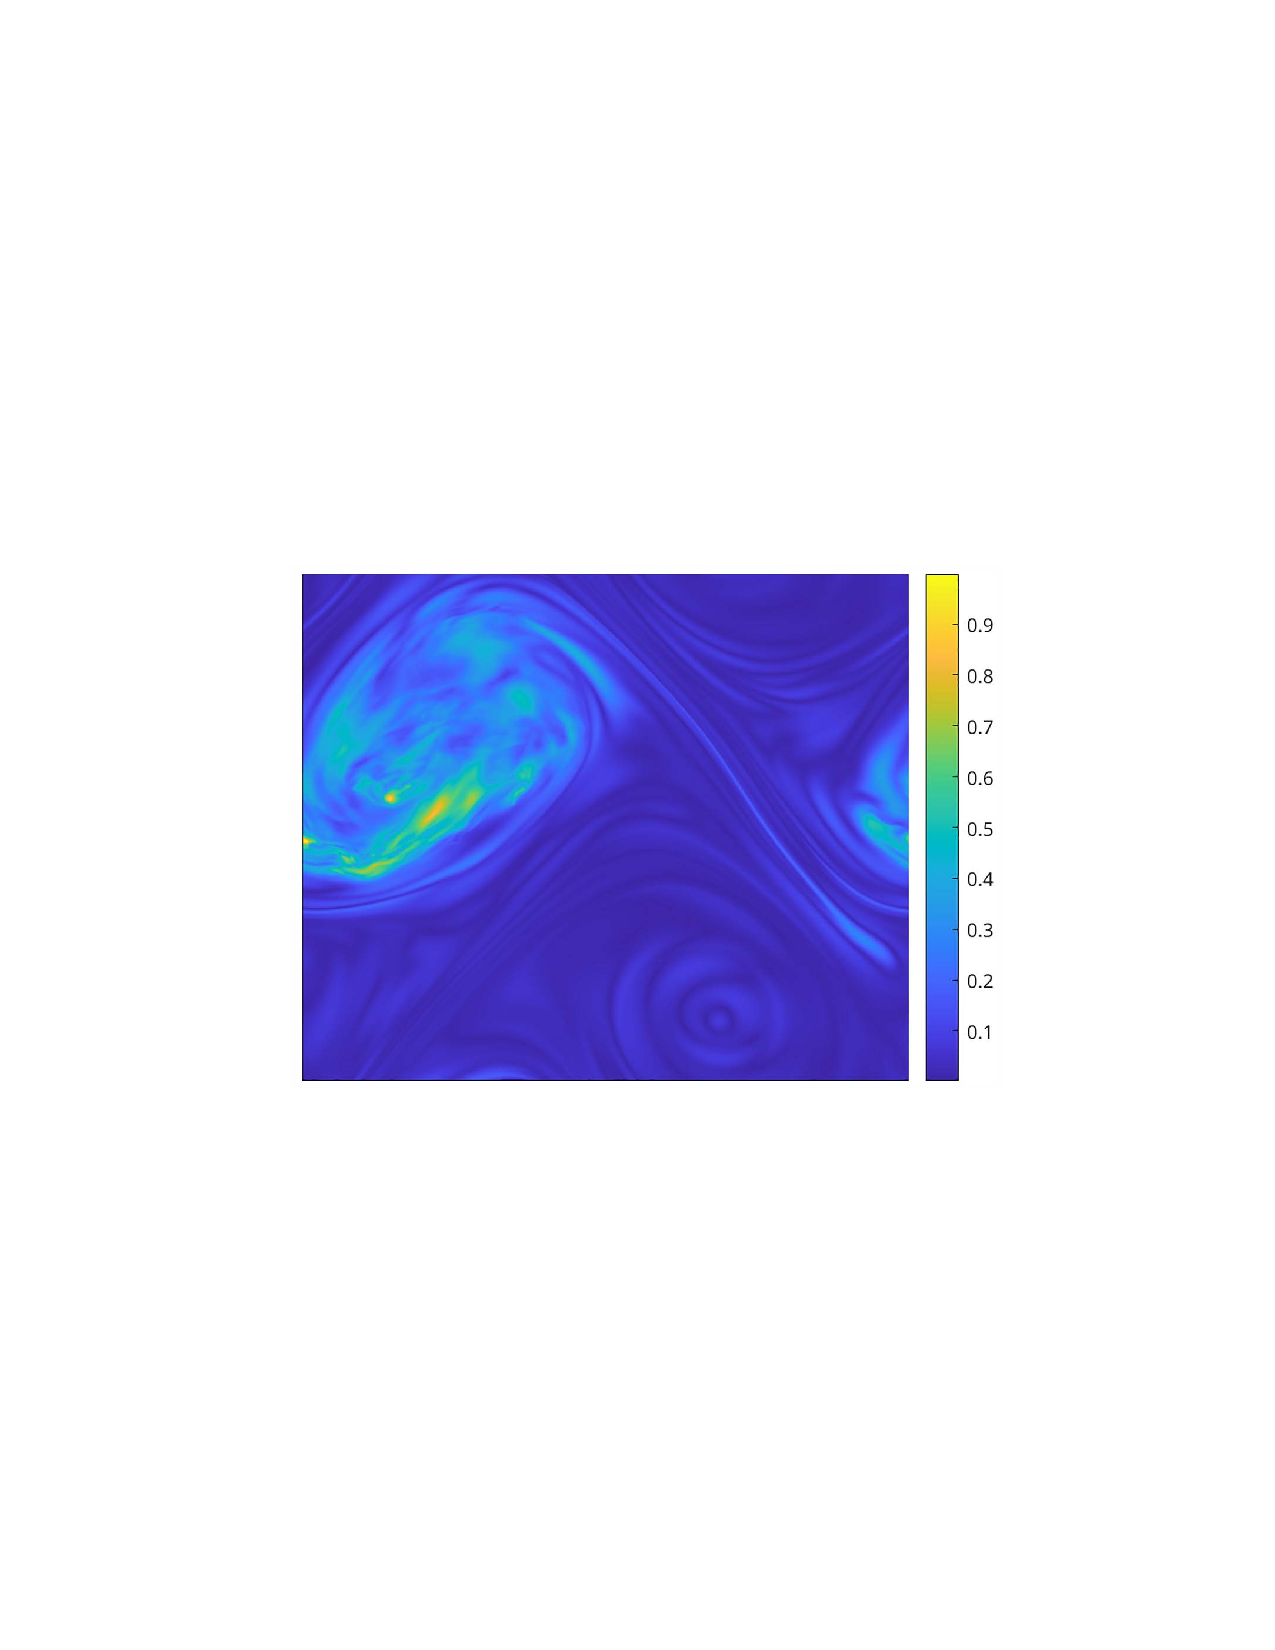
\includegraphics[width=1\textwidth]{images/Om10B30_uzrms_bar.pdf}
    \emp

\end{frame}

\begin{frame}{Temperature Transport and Mixing in the Flow}
    \bmp{.49}
        % buoyancy flux
        \centering
        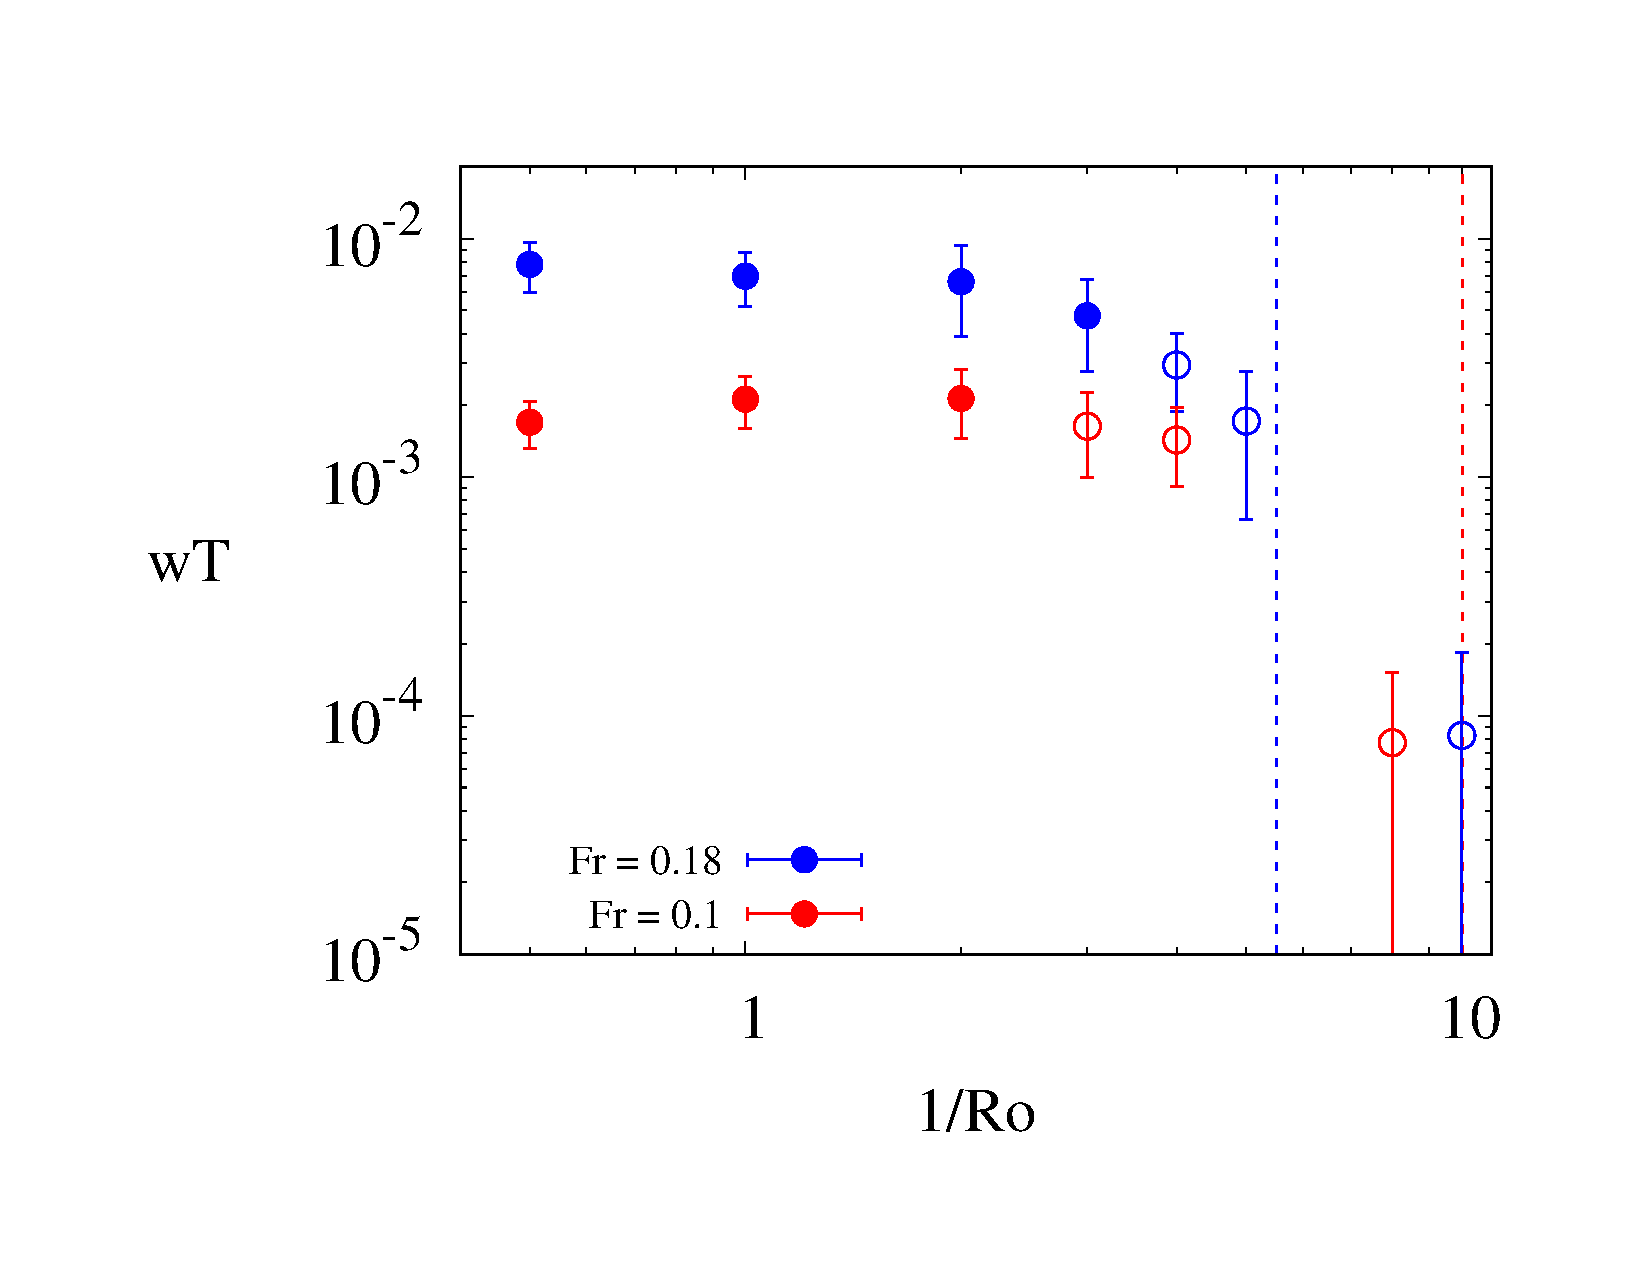
\includegraphics[width=1\textwidth]{images/bflux_plot.pdf}
    \emp
    \bmp{.49}
        % eta
        \centering
        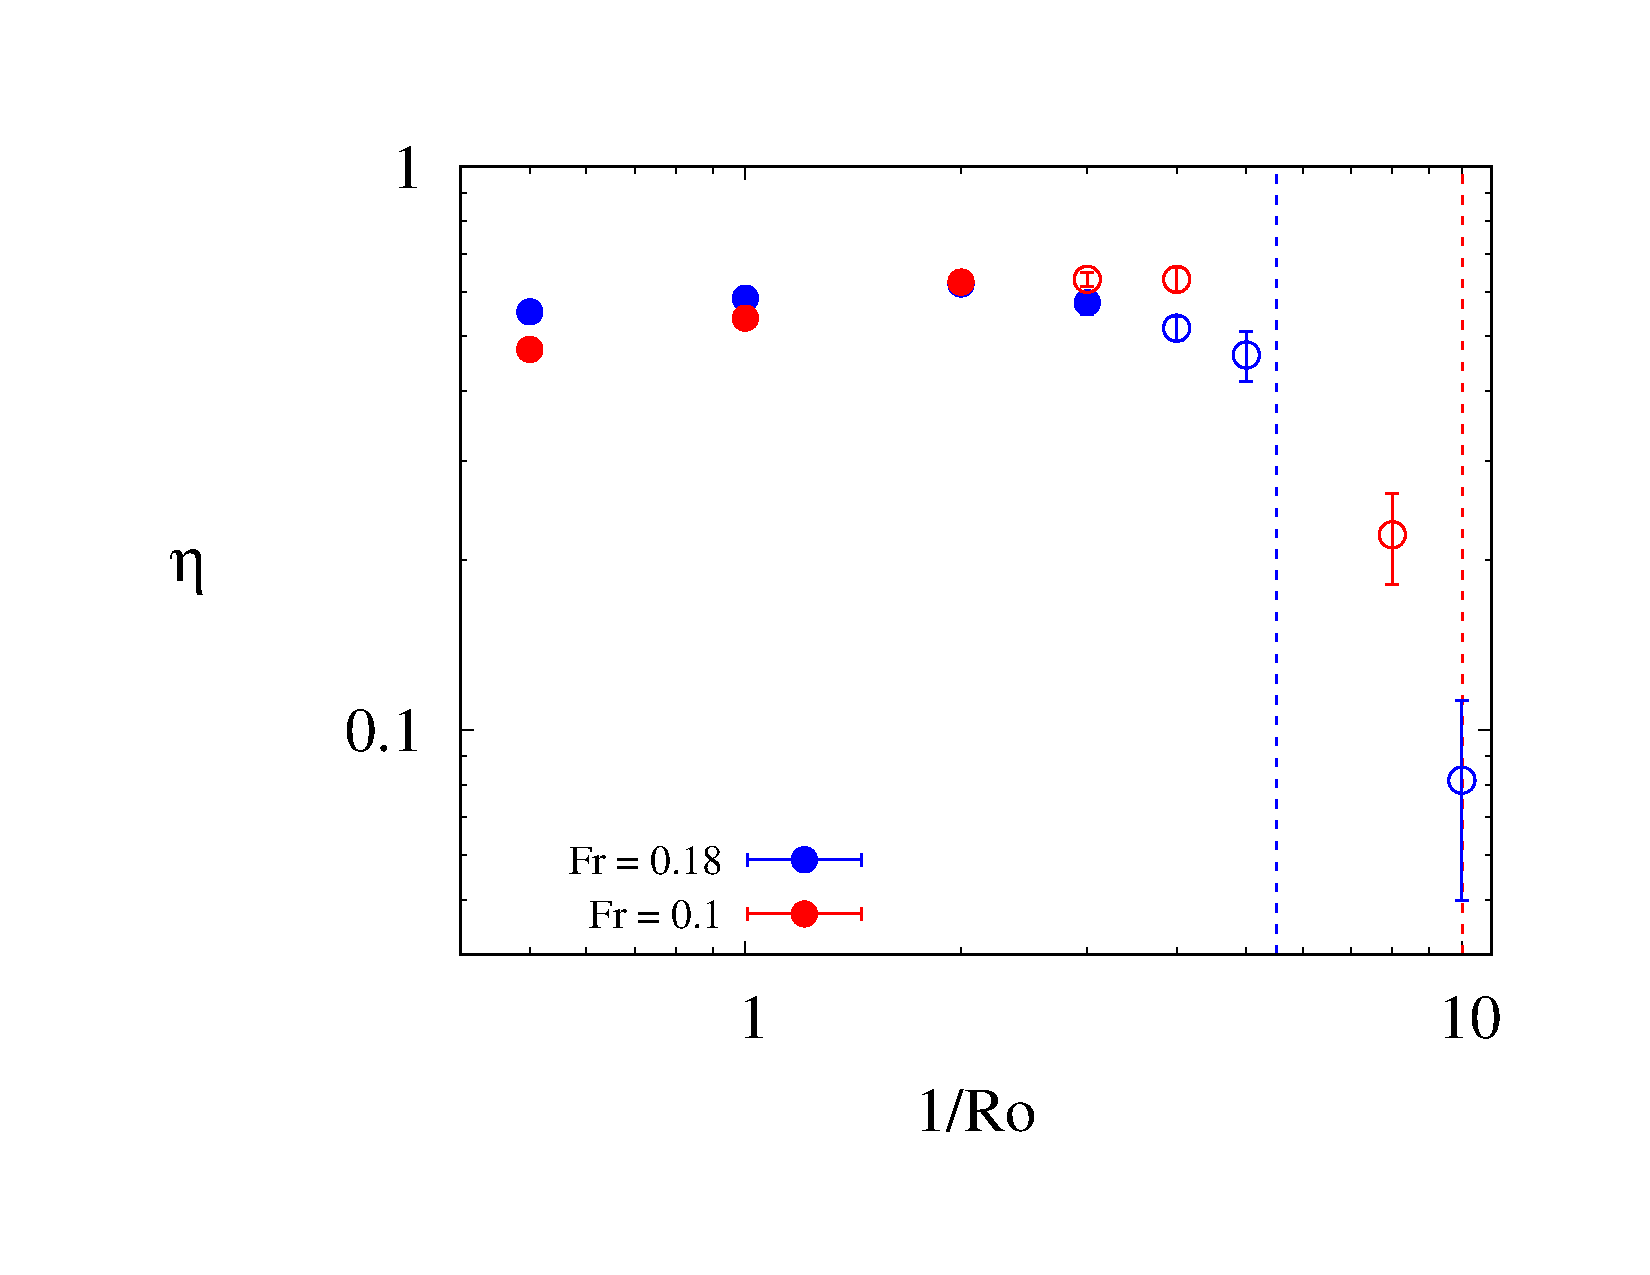
\includegraphics[width=.91\textwidth]{images/mixing_plot.pdf}
    \emp

    \vspace{10pt}

    \bmp{.49}
        \[\left< \bs{F}\cdot \uvec\right> = -\frac{\left<wT\right>}{Fr^2} +
        \frac{\left<|\grad \uvec|^2\right>}{Re}\]
        \[ -\left<wT\right> = \frac{\left<|\grad T|^2\right>}{Pe}\]
    \emp
    \bmp{.49}
         \[\eta = \frac{\frac{\left<|\grad
         T|^2\right>}{Fr^2Pe}}{\frac{\left<|\grad T|^2\right>}{Fr^2Pe} +
        \frac{\left<|\grad \uvec|^2\right>}{Re}}
        \]
    \emp
\end{frame}


%\begin{frame}{Mixing and Vertical Vorticity}
    %\centering
    %\bmp{0.07}
        %$\omega_z$

        %\vspace{75pt}

        %$\frac{|\nabla T|^2}{Pe}$
    %\emp
    %\bmp{0.31}
        %\centering
        %$1/Ro = 1$
        %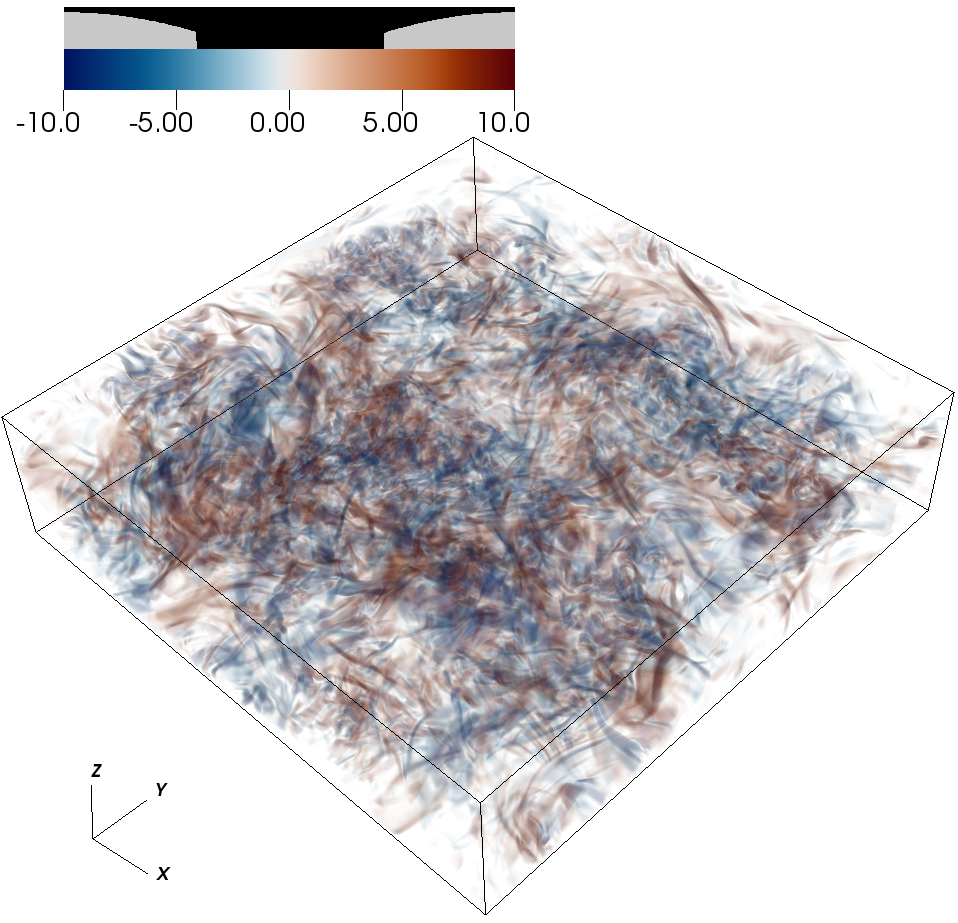
\includegraphics[width=.95\textwidth]{images/vortz_Om0.5_vr2.png}
        %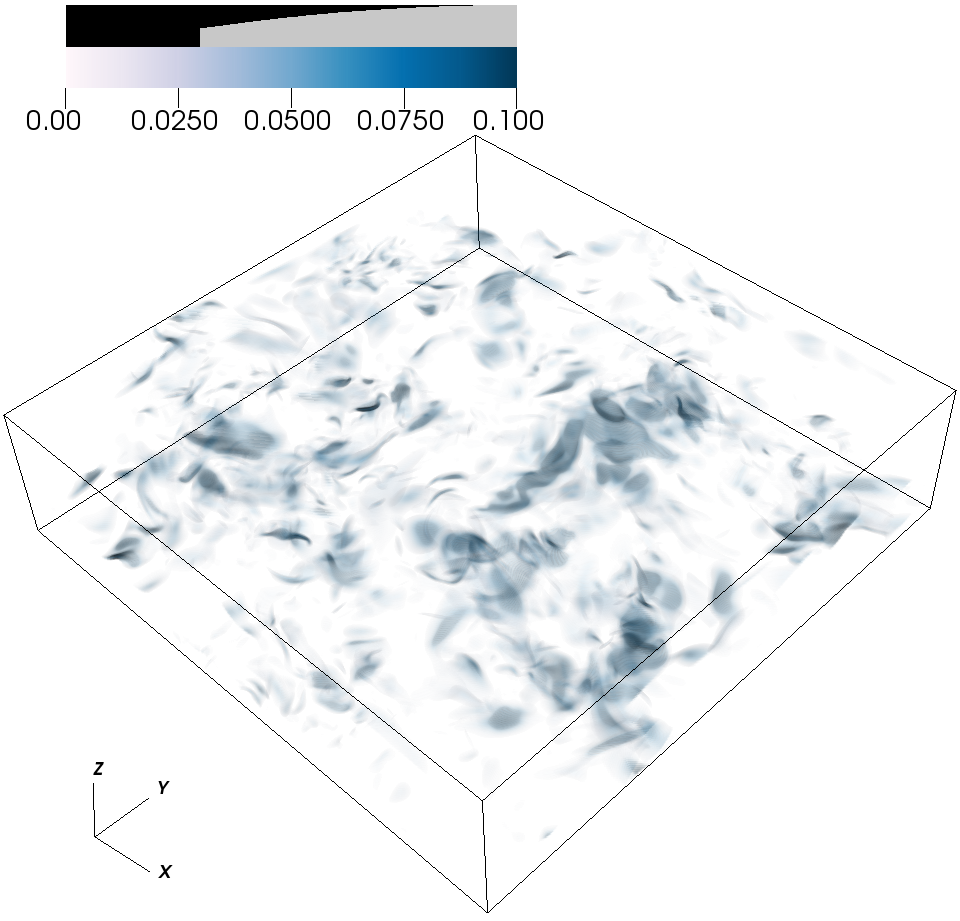
\includegraphics[width=.95\textwidth]{images/chi_Om0.5_vr2.png}
    %\emp
    %\bmp{0.31}
        %\centering
        %$1/Ro = 2$
        %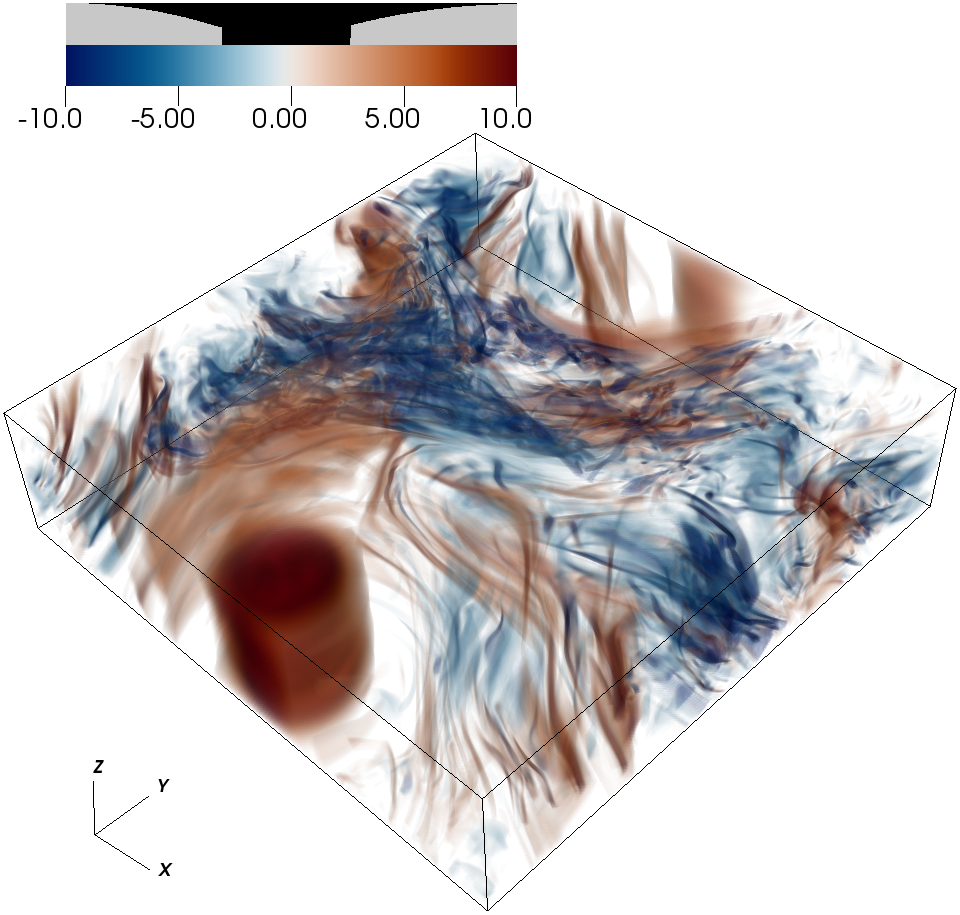
\includegraphics[width=.95\textwidth]{images/vortz_Om2_vr2.png}
        %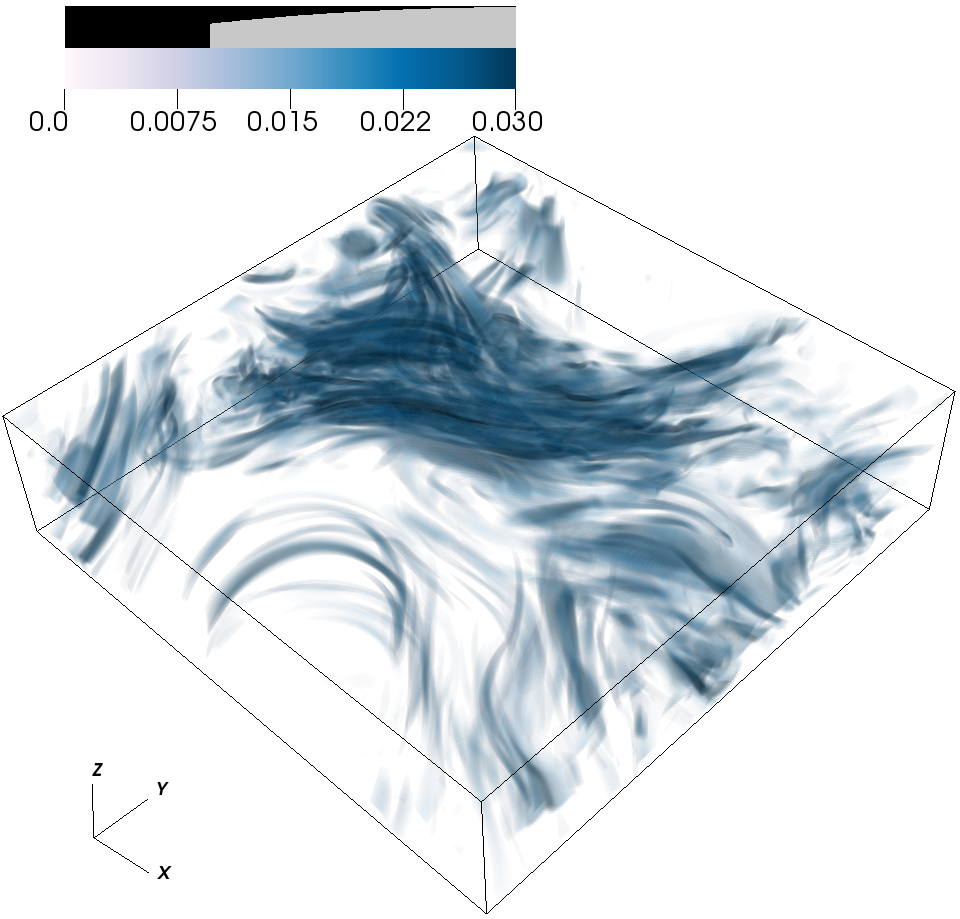
\includegraphics[width=.95\textwidth]{images/chi_Om2_vr2.png}
    %\emp
    %\bmp{0.31}
        %\centering
        %$1/Ro = 10$
        %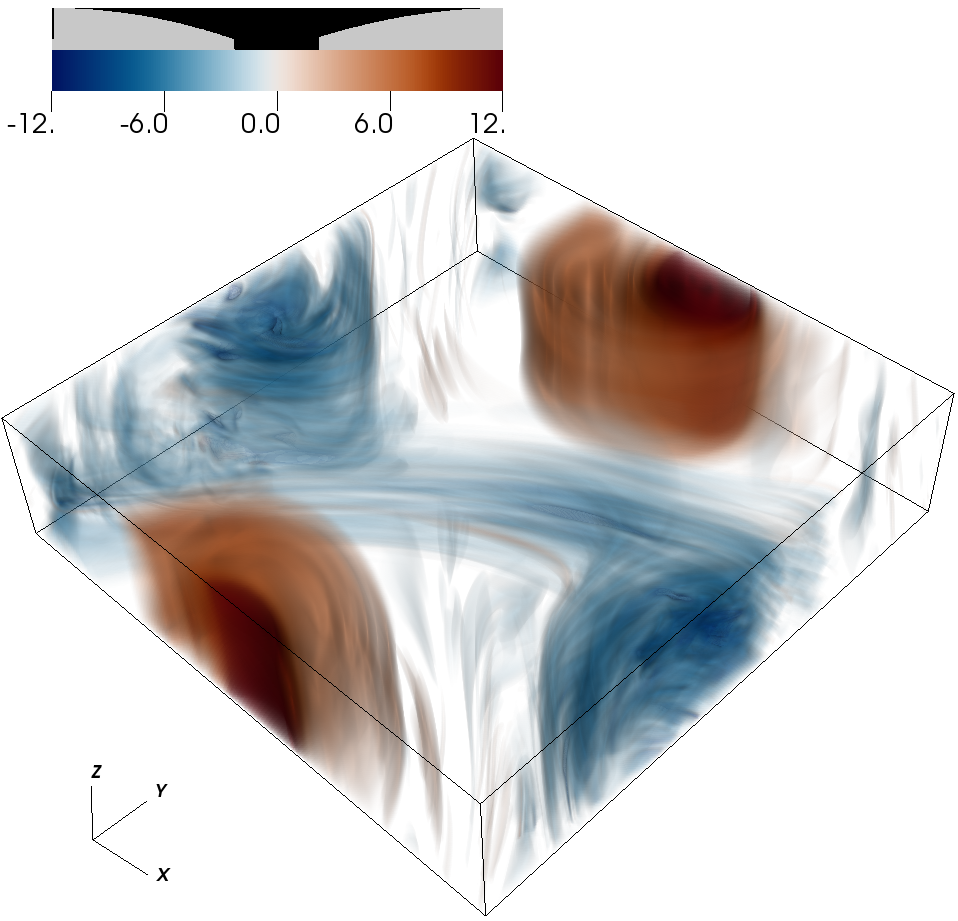
\includegraphics[width=.95\textwidth]{images/vortz_Om10_vr2.png}
        %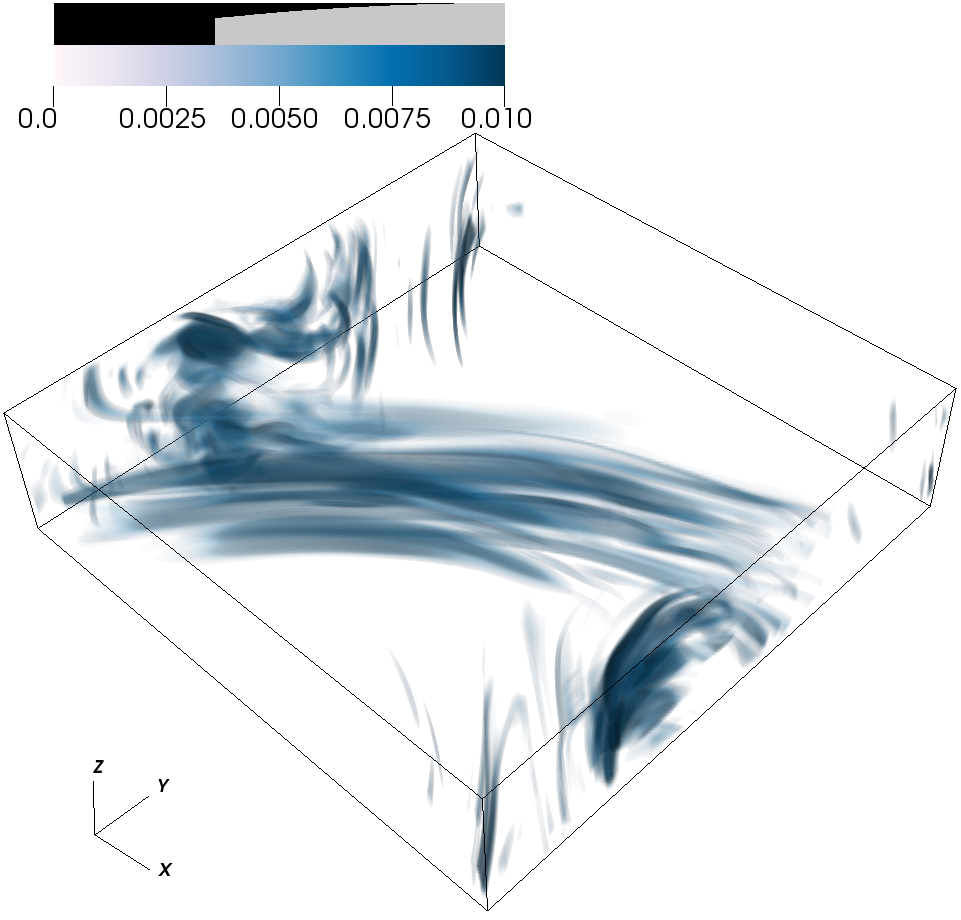
\includegraphics[width=.95\textwidth]{images/chi_Om10_vr2.png}
    %\emp

%\end{frame}

\begin{frame}{Correspondance between Planetary Vorticity and Mixing}

    \centering
    \bmp{.1}
        \centering
        {\footnotesize $\widehat{\omega_z} + Ro^{-1}$}
    \emp
    \bmp{.3}
        \centering
        $1/Ro = 1$
        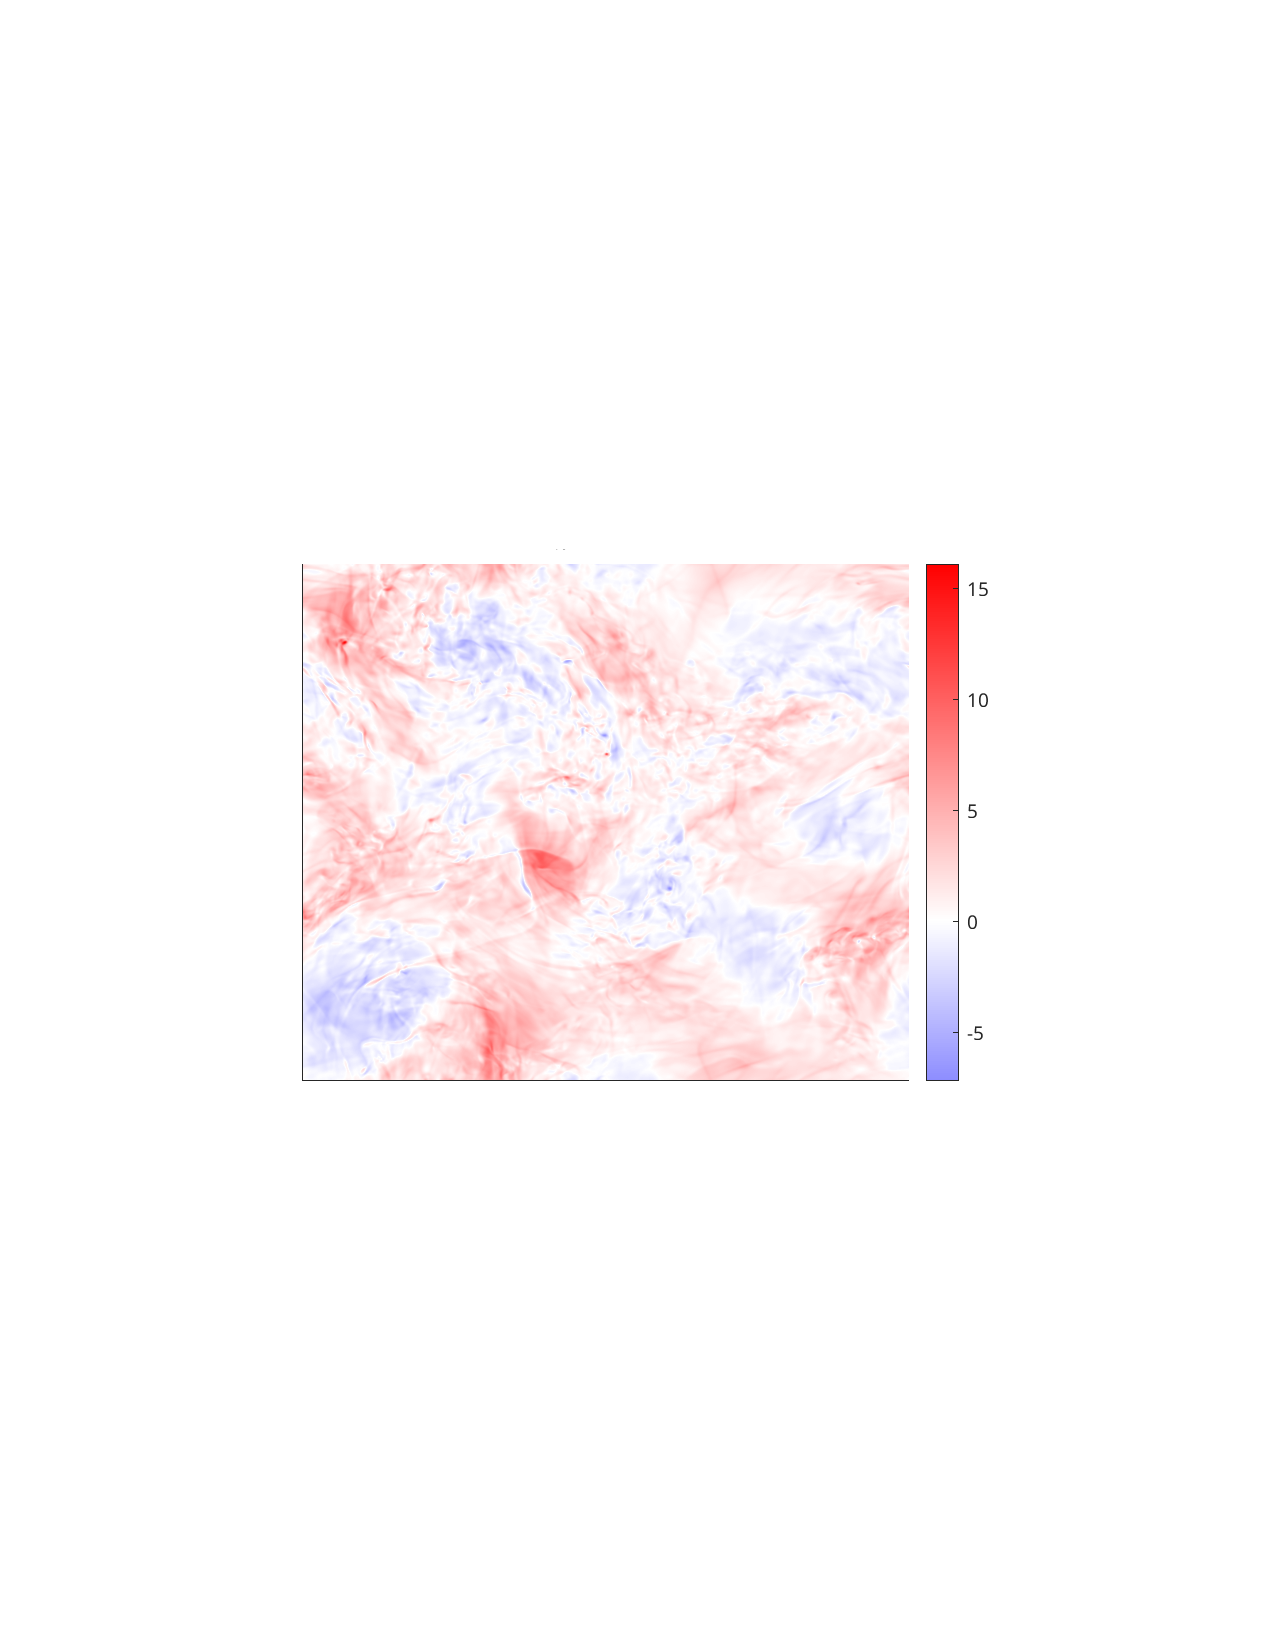
\includegraphics[width=1\textwidth]{images/Om1B30_vortz_bar.pdf}
    \emp
    \bmp{.3}
        \centering
        $1/Ro = 3$
        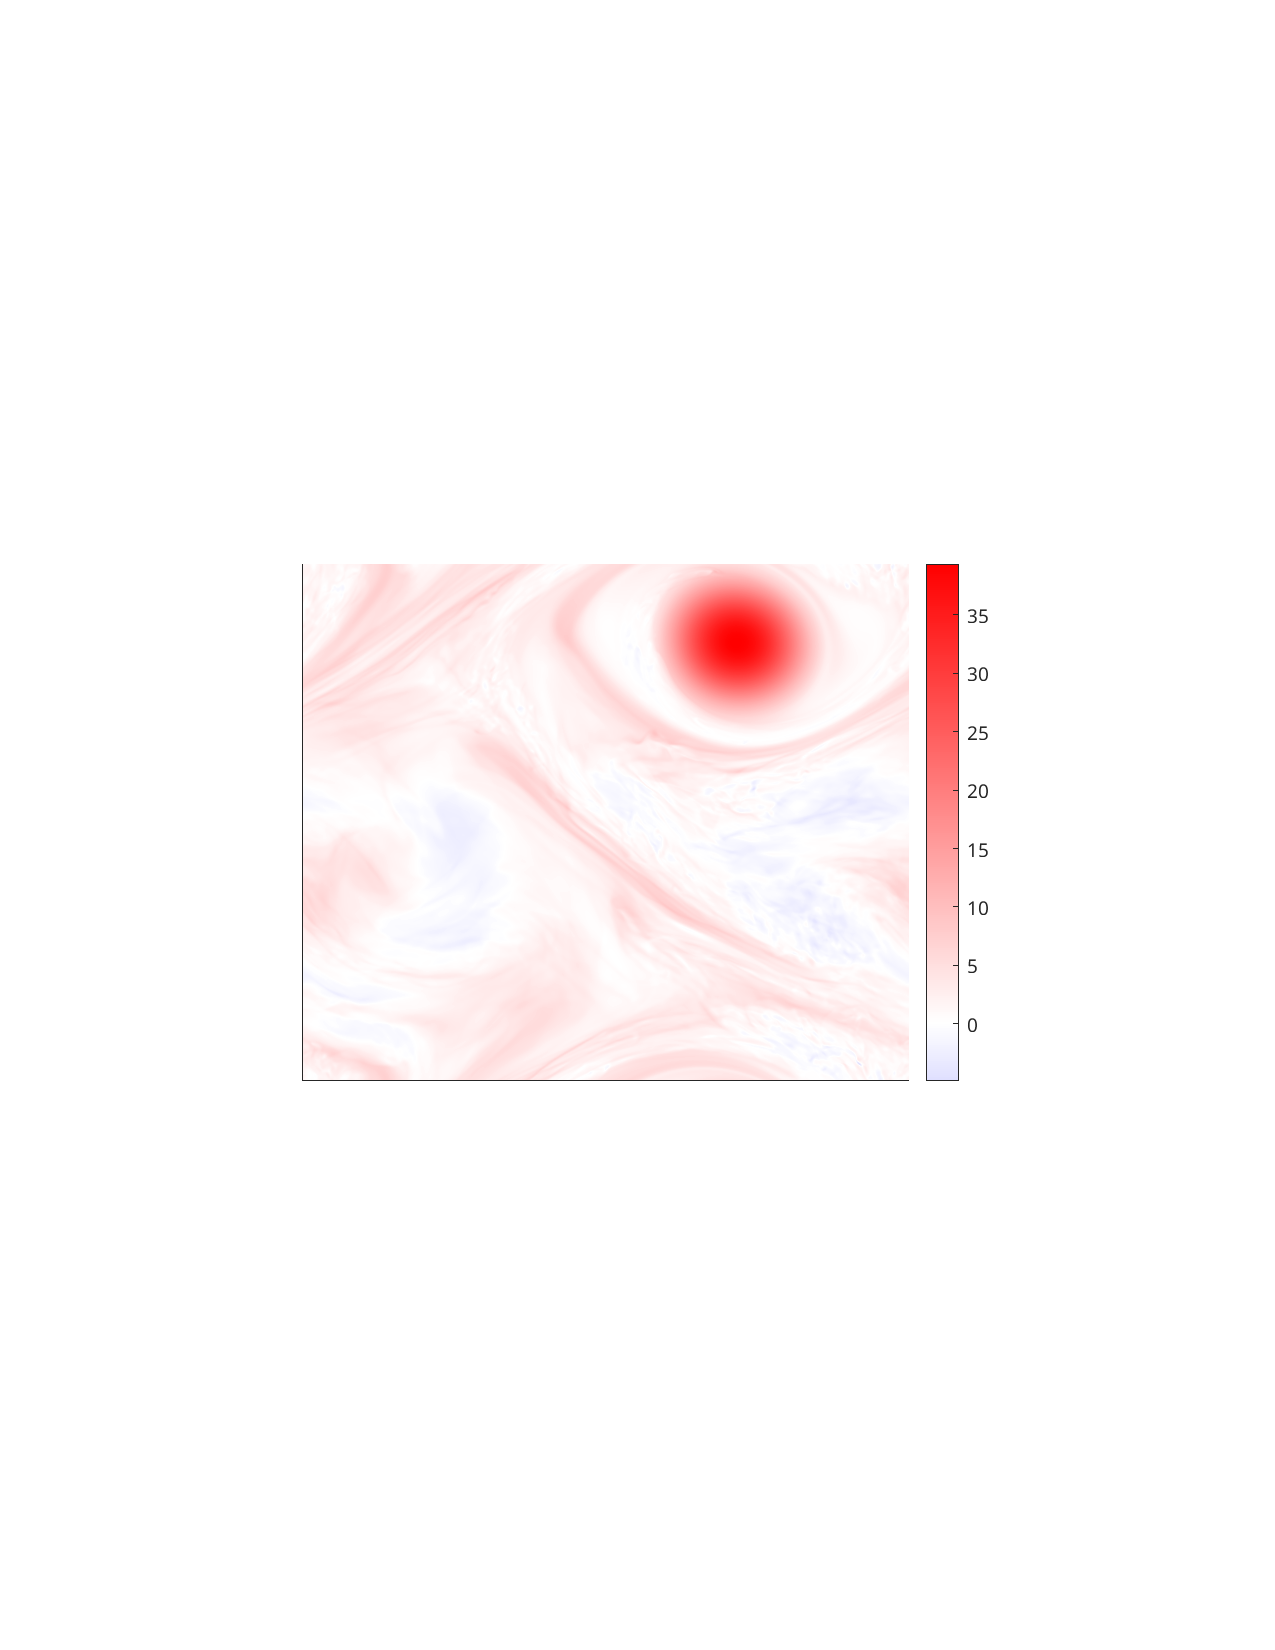
\includegraphics[width=1\textwidth]{images/Om3B30_vortz_bar.pdf}
    \emp
    \bmp{.3}
        \centering
        $1/Ro = 10$
        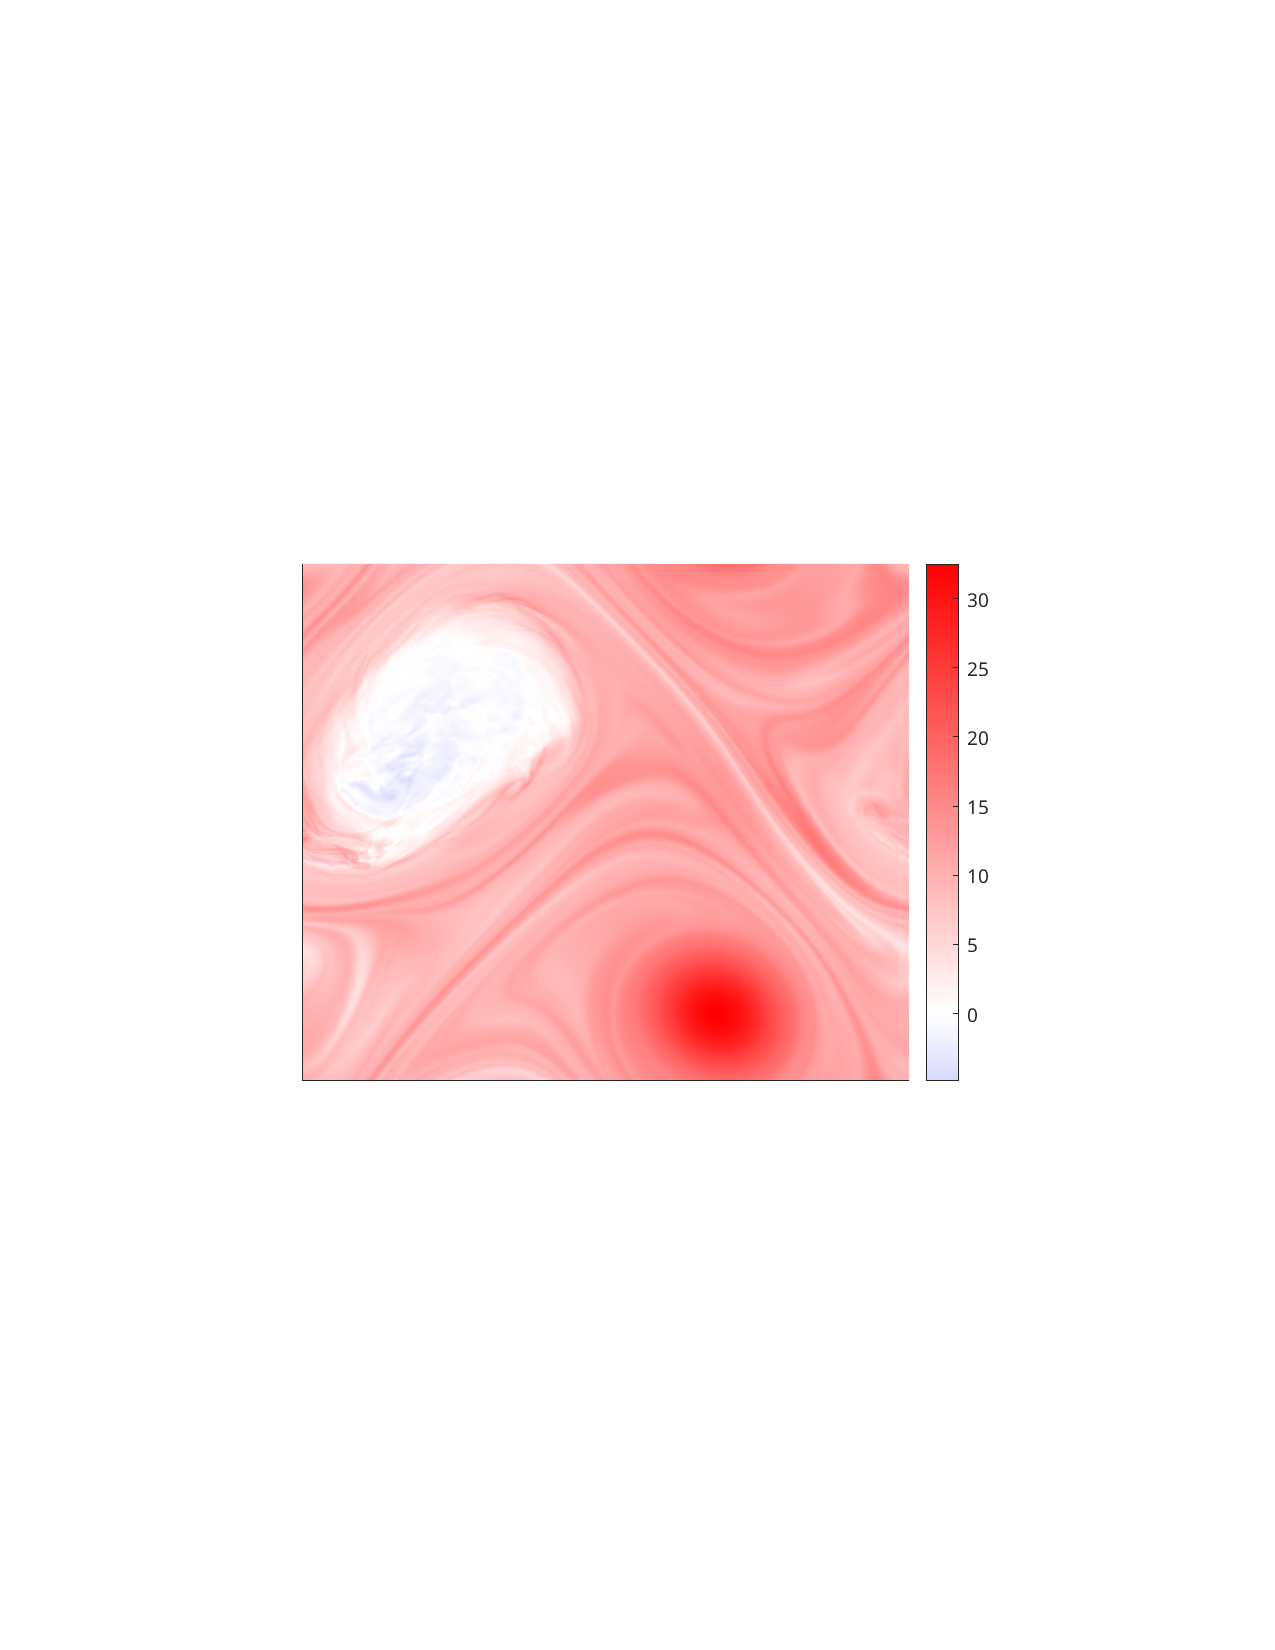
\includegraphics[width=1\textwidth]{images/Om10B30_vortz_bar.pdf}
    \emp

    \bmp{.1}
        \centering
        {\footnotesize $\frac{\widehat{|\grad T|^2}}{Fr^2Pe}$}
    \emp
    \bmp{.3}
        \centering
        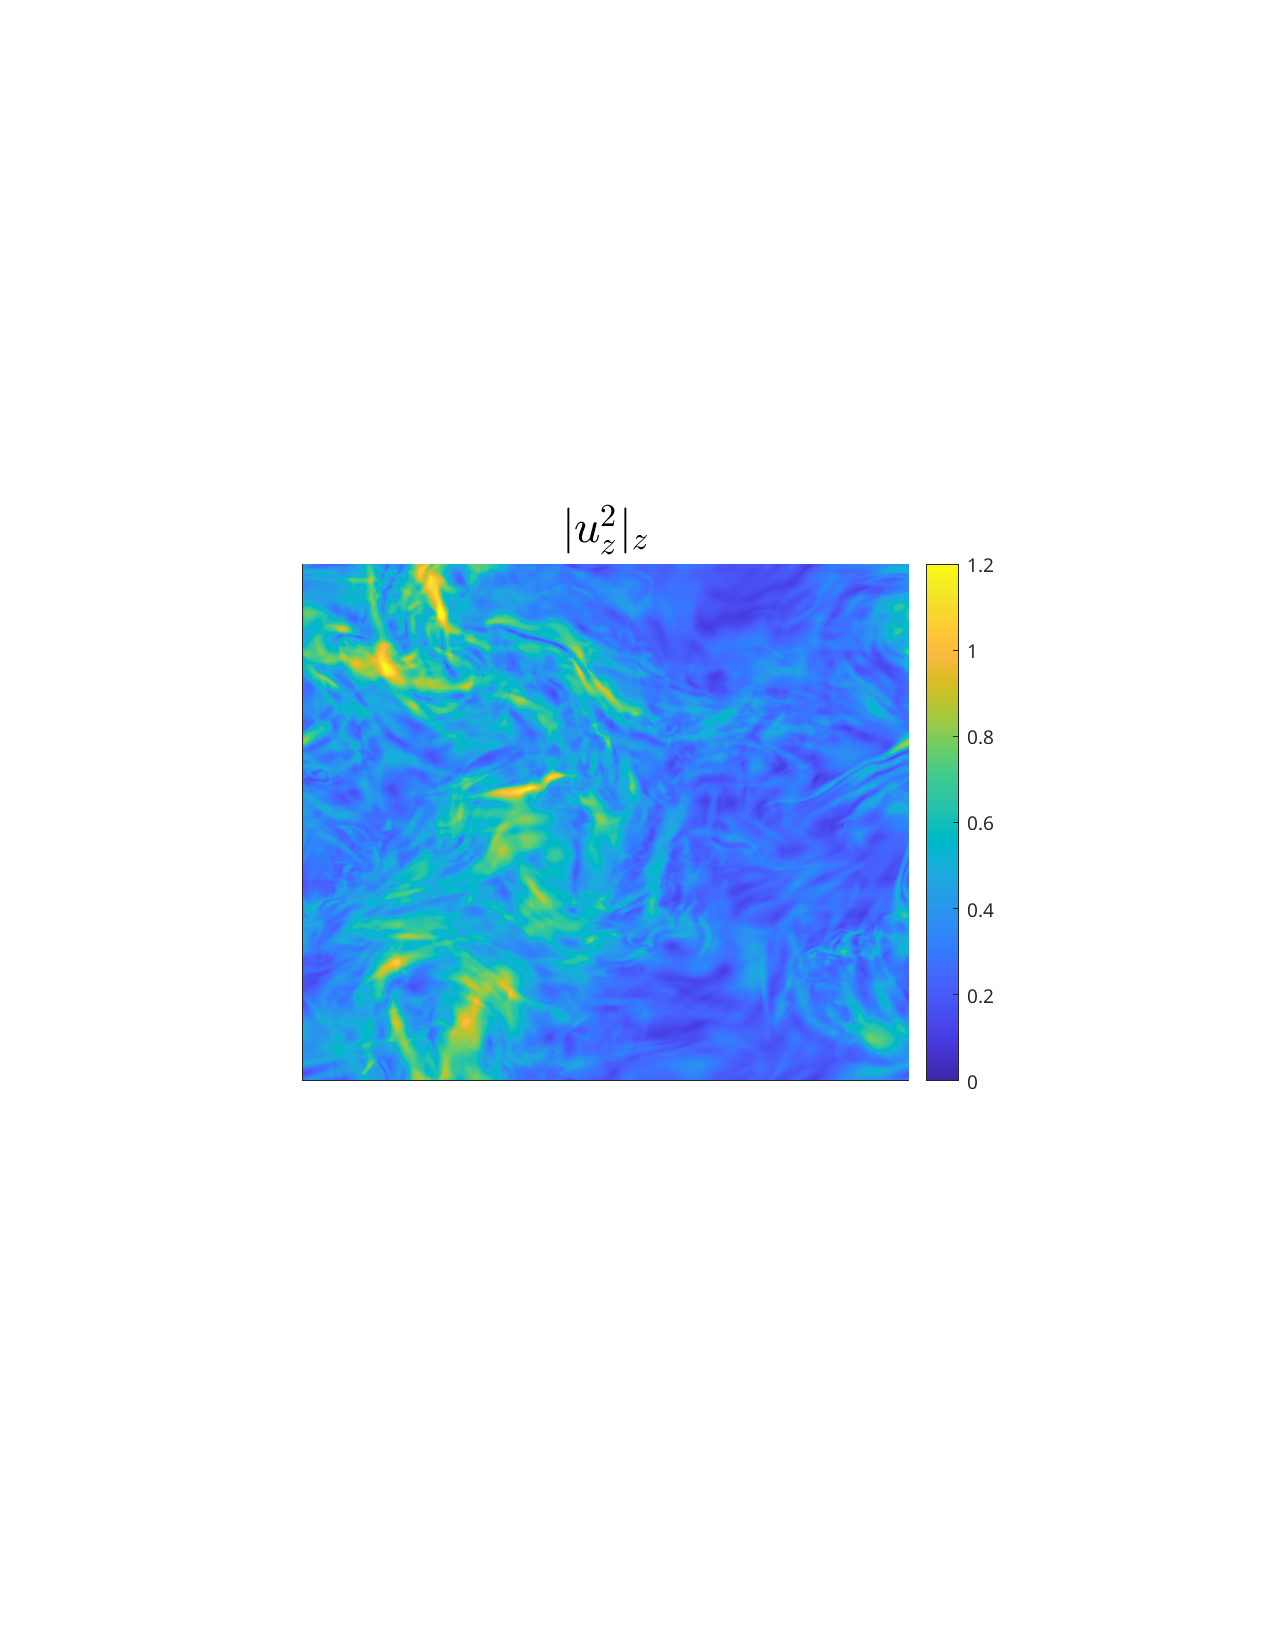
\includegraphics[width=1\textwidth]{images/Om1B30_uzrms_bar.pdf}
    \emp
    \bmp{.3}
        \centering
        \includegraphics[width=1\textwidth]{images/Om3B30_uzrms_bar.pdf}
    \emp
    \bmp{.3}
        \centering
        \includegraphics[width=1\textwidth]{images/Om10B30_uzrms_bar.pdf}
    \emp

\end{frame}


\begin{frame}{Summary}

    \begin{itemize}
    \item For $Ro > 1$, no significant change from the non-rotating case
    \item For $1 > Ro > Fr$, horizontal flow becomes increasingly
    two-dimensional, and vertical mixing is localized in regions of low total
    vorticity. 
    \item In particular, for low $Ro$ the cyclones are especially stable due to
    a high total planetary vorticity. Mixing is localized outside of these
    vortices. 
    \item $\eta$ is approximately constant for $Ro > Fr$. 
    \end{itemize}

\end{frame}

\end{document}
